\chapter{Introduction}\label{introduction}

\section{The clinical problem}\label{the-clinical-problem}

Ovarian cancer continues to pose a major challenge to global health. Data from the IARC GLOBOCAN report establishes a heavy global baseline with an estimated 324,603 women diagnosed with the disease worldwide in a single year (Bray et al., 2024) and long-term projections estimating a near 47\% increase in global burden by 2050. Because early symptoms are frequently nonspecific, most patients present with advanced disease. This late presentation is associated with reduced survival and places considerable weight on initial treatment decisions. Historically, the standard approach relied on primary cytoreductive surgery followed by adjuvant chemotherapy. More recently, consensus has shifted toward neoadjuvant chemotherapy with carboplatin and paclitaxel prior to interval surgery for advanced disease to improve operability and perioperative outcomes (ASCO, 2025; Colombo et al., 2019). Nevertheless, response to these regimens remains highly heterogeneous. While some individuals experience complete remission, others see their disease progress within months meaning they endure severe side effects for little to no clinical return.

The core problem this thesis tackles is not a biological mystery but an informational one. Right now clinical guidelines depend on population averages from clinical trials. By design these averages cannot predict how a specific individual will react to a drug. While a solid prognostic model can tell us \emph{who} is likely to have a good outcome, it cannot prove whether the treatment itself actually caused that success (Obermeyer and Emanuel, 2016). This gap between prediction and causation has real-world consequences for patient well-being. For instance, Prigerson et al. (2015) demonstrated that aggressive chemotherapy near the end of life frequently erodes a patient\textquotesingle s quality of life without offering any survival advantage. Wright et al. (2016) noted similar clinical missteps when doctors lacked specific information on individual treatment effects.

Precision oncology has tried to bridge this divide through functional testing, using tools like patient derived xenografts (Gao et al., 2015) and organoid assays (Pauli et al., 2017). The science behind these methods is promising but practical access is restricted to a handful of elite academic medical centers. A patient living in a rural area or relying on a regional hospital rarely has a realistic path to organoid guided care, a disparity that worsens along racial and geographic lines. Furthermore, these inequities are embedded in the data itself. Landry et al. (2018) highlighted that patients of African descent are systematically left out of the genomic databases used to drive modern precision medicine.

This thesis builds on the premise that personalised cancer care should not depend on access to specialised research infrastructure. This is increasingly salient as treatment decisions are made earlier in the care pathway, often before surgical tissue is available. If routinely collected clinical data contain sufficient signal to capture heterogeneity in treatment response, then developing a causal inference pipeline around these existing variables represents a substantive contribution.

\section{Why existing AI systems fall short}\label{why-existing-ai-systems-fall-short}

Machine learning has made substantial progress in predicting ovarian cancer outcomes. Models including XGBoost classifiers, Random Survival Forests and Cox regression have demonstrated accurate stratification of patients into risk categories in validation studies. Several such models have progressed to prospective evaluation for trial eligibility screening.

The central limitation is not the statistical method itself but its application to causal questions. Predicting which patients are likely to live longer addresses an observational question, whereas determining whether a specific therapy will benefit a particular individual addresses a causal question. Conflating survival prediction with treatment benefit risks severe algorithmic bias, as illustrated by Obermeyer et al. (2019) in a widely deployed healthcare risk model that inadvertently disadvantaged vulnerable patient groups.

A further barrier concerns trust and explainability. Clinicians are appropriately cautious in adopting algorithmic recommendations when model reasoning is opaque and difficult to interrogate. In parallel, the regulatory environment has undergone substantial change. Under Regulation (EU) 2024/1689, commonly referred to as the EU Artificial Intelligence Act, AI systems intended for clinical decision support are classified as high risk applications (European Parliament and Council, 2024; Hacker et al., 2024). This classification imposes binding requirements relating to data governance, technical documentation, transparency, human oversight, cybersecurity and robustness. Because the majority of existing clinical AI tools were developed prior to the finalisation of these provisions, few were designed to satisfy this level of accountability at inception.

\section{What this thesis contributes}\label{what-this-thesis-contributes}

CaML-OP combines gradient boosted prognostic encoding with causal meta learning to estimate individualized treatment effects for platinum chemotherapy from routine clinical data. An XGBoost model is first trained on binary five year survival. Its terminal leaf assignments are extracted to capture nonlinear prognostic structure and subsequently provided as augmented features to an R-Learner and a Doubly Robust Learner. The final estimate is the equally weighted mean of the two causal estimators, which stabilises performance across heterogeneous effect structures.

An explainability layer complements the estimator. Effect-SHAP attributes variation in the estimated treatment effect function rather than variation in predicted survival, thereby isolating causal drivers. A large language model module translates these quantitative outputs into concise clinical summaries that are subject to automated faithfulness verification prior to display.

The interface is designed to be informed by the EU Artificial Intelligence Act high risk framework. Per patient explanations, calibrated uncertainty communication and subgroup reporting are implemented as design responses to the principles of the regulation. The system is therefore AI Act informed rather than legally deployment ready, and no claim of conformity or certification is made.

The remainder of the thesis tests this architecture. A semi-synthetic benchmark pairs real TCGA-OV data with simulated outcomes across four scenarios to evaluate CaML-OP against nine baseline models. Over forty tests are conducted followed by a synthetic verification of statistical consistency.

\section{Research questions}\label{research-questions}

The main question is whether a hybrid predictive causal pipeline can generate useful individualized treatment-effect estimates for platinum chemotherapy in ovarian cancer using only standard clinical variables.

\textbf{1.4.1 Objectives}

\begin{itemize}
\item
 \textbf{O1:} Build a causal ITE estimation pipeline on TCGA-OV data that uses XGBoost leaf embeddings as features for R- and DR-Learner estimators. Then validating it via semi-synthetic benchmarks.
\item
 \textbf{O2:} Benchmark CaML-OP against three binary outcome predictive models and five causal meta-learners to evaluate ITE accuracy and off policy value.
\item
 \textbf{O3:} Deploy an Effect-SHAP attribution layer and an LLM narrative module with automated accuracy checks.
\item
 \textbf{O4:} Show end-to-end functionality through a dashboard prototype featuring subgroup error reporting and a built-in transparency card.
\end{itemize}

\textbf{1.4.2 Secondary Questions}

\begin{itemize}
\item
 \textbf{RQ1:} How varied are the estimated platinum therapy effects across subgroups (age, FIGO stage, race), and which covariates drive treatment benefit the most?
\item
 \textbf{RQ2:} Can LLM-generated summaries stay entirely faithful to underlying numeric causal data while remaining easy for clinicians to read?
\item
 \textbf{RQ3:} Are there noticeable differences in ITE estimation errors across demographic subgroups on this benchmark that require deeper investigation?
\end{itemize}

\section{Thesis structure}\label{thesis-structure}

Chapter 2 reviews the relevant literature and establishes how CaML-OP builds on existing research. Chapter 3 breaks down the technical components of the pipeline itself. Chapter 4 outlines the experimental design and Chapter 5 present the empirical findings. Finally, Chapter 6 discusses the broader implications of these results, addresses the core research questions and explores ethical concerns alongside threats to validity, leading into concluding remarks in Chapter 7.

\chapter{Related Work}\label{related-work}

\section{Predictive survival modelling}\label{predictive-survival-modelling}

For decades the Cox proportional hazards model (Cox, 1972) has been the bedrock of oncology survival analysis. It remains popular because hazard ratios are easy to interpret, the model is widely understood and it holds up reasonably well even when its core proportional hazards assumption is slightly violated. Random Survival Forests (Ishwaran et al., 2008) step past this limitation by handling non-linear covariate effects and consistently outperforming Cox models when feature interactions are highly complex. While XGBoost (Chen and Guestrin, 2016) is typically used for standard tabular classification rather than survival tracking. It performs competitively when applied to binary survival endpoints. In fact, Yin et al. (2022) proved its utility specifically for ovarian cancer prognosis.

However, all these methods share a fundamental bottleneck. They are strictly correlative. A survival model tells us that patients with a specific set of traits tend to experience specific outcomes. What it cannot tell us is whether a chosen patient\textquotesingle s outcome would actually change if she received platinum therapy versus if she did not. Treating a correlation as a cause can lead to genuine patient harm. A risk starkly illustrated by Obermeyer et al. (2019) when a massive, real-world clinical risk algorithm inadvertently used healthcare spending as a proxy for actual medical need. To address this CaML-OP includes Cox PH and a Random Forest classifier strictly as binary-outcome predictive comparators rather than full time-to-event survival baselines. The exact implications of this decision on construct validity are explored later in Section 6.7.3.

\section{Causal ML for treatment effect heterogeneity}\label{causal-ml-for-treatment-effect-heterogeneity}

Traditional meta-learners like the T-Learner, S-Learner, and X-Learner (Künzel et al., 2019) turn this theory into practical code, though their performance varies depending on treatment imbalances and how well the nuisance models are specified.

To handle these challenges more robustly, the R-Learner (Nie and Wager, 2021) leverages Robinson\textquotesingle s (1988) partial-linear decomposition to create a Neyman-orthogonal loss function. This orthogonality is a major advantage. It ensures that first-order mistakes in your nuisance models only cause minor, second-order errors in the final ITE estimate. Similarly, the DR-Learner (Kennedy, 2023) builds in robustness by using doubly robust pseudo-outcomes, which stay accurate as long as either the outcome model or the propensity score model is correct.

CaML-OP combines these two approaches into an equally weighted ensemble. Because each learner handles nuisance errors differently, combining them makes the overall system far more stable across different clinical scenarios. To keep the evaluation grounded, a Causal Forest (Wager and Athey, 2018) is added as a standalone baseline. It uses honest estimation to generate valid confidence intervals making it the perfect benchmark for testing CaML-OP\textquotesingle s uncertainty reporting.

\section{Benchmarking ITE estimators}\label{benchmarking-ite-estimators}

Curth et al. (2021a) published a vital critique regarding how heterogeneous treatment effect (HTE) benchmarks are typically run. Two of their insights directly shaped the evaluation structure of this thesis. First they noted that published comparisons often evaluate different methods under completely inconsistent conditions which makes it nearly impossible to tell if one algorithm is truly better than another. Second they found that a model\textquotesingle s PEHE rank is a poor predictor of how well it actually guides clinical choices. A method with a slightly better PEHE score doesn\textquotesingle t automatically mean it will recommend therapies to the right patients. This thesis directly controls for both issues. Finally, while Curth et al. (2021b) also introduced SurvITE specifically to handle time-to-event HTE estimation, this project opts for a binary outcome at a fixed horizon to keep the pipeline practical and mathematically tractable.

\section{Explainability and the EU AI Act}\label{explainability-and-the-eu-ai-act}

The EU AI Act officially Regulation (EU) 2024/1689 was adopted in 2024 and officially took effect on August 1st of that year. Under Annex III of the law, AI systems deployed for medical purposes are strictly classified as "high-risk." This label binds developers to rigorous standards regarding data governance, detailed technical documentation, transparency for users, and strong human oversight. This thesis builds entirely on that exact perspective.

On the explainability side, SHAP (Lundberg and Lee, 2017; Lundberg et al., 2020) stands as the gold standard for pulling post-hoc insights out of complex machine learning models. However using it in medicine requires care. Reyes et al. (2020) evaluated interpretability in radiology AI and highlighted how easily clinicians can misinterpret these tools depending on how the data is presented. In the case of CaML-OP running standard SHAP on the initial survival predictor would completely miss the mark by explaining the wrong target entirely. To fix this the pipeline introduces Effect-SHAP, which directly calculates attributions for the ITE function itself. This shifts the focus entirely to the causal treatment effect, ensuring the explanation targets the exact clinical decision a doctor needs to make.

\section{LLMs in clinical settings}\label{llms-in-clinical-settings}

Large language models have been studied in medical settings with mixed results. Tayebi Arasteh et al. (2024) demonstrated that LLMs can streamline aspects of automated machine learning for clinical studies. Hallucination remains a serious concern (Thirunavukarasu et al., 2023). Rather than fine-tuning an LLM, CaML-OP constrains the prompt to provide only numeric model outputs and runs automated consistency checks on every generated narrative before display. This adequately controls hallucination risk is discussed in Chapter 6.

\section{Platinum response heterogeneity in HGSOC}\label{platinum-response-heterogeneity-in-hgsoc}

Platinum sensitivity is the dominant prognostic factor after cytoreduction in ovarian cancer. Hanker et al. (2012) reported median overall survival of approximately 56.6, 27.0 and 11.6 months for platinum-sensitive, platinum-resistant and platinum-refractory disease respectively. The biological underpinnings involve BRCA1/2 mutations, homologous recombination deficiency and DNA damage repair pathway alterations (Shenoy et al., 2020). Kilim et al. (2025) recently showed that multimodal deep learning integrating histopathology and proteomics predicts platinum response in HGSOC, but the approach requires whole-slide imaging and proteomic mass spectrometry, which are not in routine clinical use.

CaML-OP is positioned differently: it accepts lower expected accuracy in exchange for requiring only variables already recorded in standard clinical records, with a view to potential deployability in facilities without specialized infrastructure.

\section{Positioning}\label{positioning}

Table 2.1 compares CaML-OP to the most relevant prior work. CaML-OP does not achieve the lowest PEHE on clean benchmarks; that distinction goes to the Causal Forest or S-Learner in some scenarios. It also does not exploit the richest available data; the Kilim et al. (2025) multimodal approach uses more information than CaML-OP can. The gap CaML-OP addresses is the intersection of causal estimation, causal explainability, and EU AI Act-informed design on routinely collected data.

\begin{longtable}[]{@{}
 >{\raggedright\arraybackslash}p{(\columnwidth - 10\tabcolsep) * \real{0.3483}}
 >{\raggedright\arraybackslash}p{(\columnwidth - 10\tabcolsep) * \real{0.0962}}
 >{\raggedright\arraybackslash}p{(\columnwidth - 10\tabcolsep) * \real{0.0962}}
 >{\raggedright\arraybackslash}p{(\columnwidth - 10\tabcolsep) * \real{0.2030}}
 >{\raggedright\arraybackslash}p{(\columnwidth - 10\tabcolsep) * \real{0.1389}}
 >{\raggedright\arraybackslash}p{(\columnwidth - 10\tabcolsep) * \real{0.1175}}@{}}
\toprule\noalign{}
\begin{minipage}[b]{\linewidth}\raggedright
\textbf{Method}
\end{minipage} & \begin{minipage}[b]{\linewidth}\raggedright
\textbf{Causal}
\end{minipage} & \begin{minipage}[b]{\linewidth}\raggedright
\textbf{Hybrid}
\end{minipage} & \begin{minipage}[b]{\linewidth}\raggedright
\textbf{XAI}
\end{minipage} & \begin{minipage}[b]{\linewidth}\raggedright
\textbf{EU AI Act}
\end{minipage} & \begin{minipage}[b]{\linewidth}\raggedright
\textbf{TCGA-OV}
\end{minipage} \\
\midrule\noalign{}
\endhead
\bottomrule\noalign{}
\endlastfoot
Kunzel et al. (2019) & Yes & No & No & No & No \\
Wager and Athey (2018) & Yes & No & Partial & No & No \\
Shalit et al. (2017) & Yes & No & No & No & No \\
Nie and Wager (2021) & Yes & No & No & No & No \\
Kennedy (2023) & Yes & No & No & No & No \\
Yin et al. (2022) & No & No & No & No & Yes \\
Kilim et al. (2025) & No & Yes & No & No & Partial \\
This thesis - CaML-OP & Yes & Yes & Yes (Effect-SHAP+LLM) & Informed & Yes \\
\end{longtable}

\setcounter{table}{0}\captionof{table}{Comparison of related methods. Causal = uses a causal identification strategy; Hybrid = combines a predictive encoder with a causal estimator; XAI = per-patient causal explanation; EU AI Act = designed with reference to Regulation (EU) 2024/1689 obligations; TCGA-OV = evaluated on TCGA-OV.}

Three gaps motivate the contribution. To my knowledge, no causal ITE benchmark for platinum therapy on TCGA-OV with semi-synthetic evaluation has been published. Existing clinical causal ML systems are not, to my knowledge, designed with reference to the obligations of Regulation (EU) 2024/1689. And the use of XGBoost leaf embeddings as features for downstream causal meta-learners has not, to my knowledge, been evaluated in an oncology context. These statements reflect a non-systematic literature search and should be read accordingly; I would welcome counter-examples that I have missed.

\chapter{Methodology}\label{methodology}

\section{Pipeline overview}\label{pipeline-overview}

CaML-OP has five stages: input, encoding, causal estimation, explainability and output. Each stage is modular, in the sense that any component can be replaced without restructuring the pipeline, and each is benchmarked against an explicit alternative in the evaluation. Figure 3.1 shows the full architecture.

\begin{figure}[H]
\centering
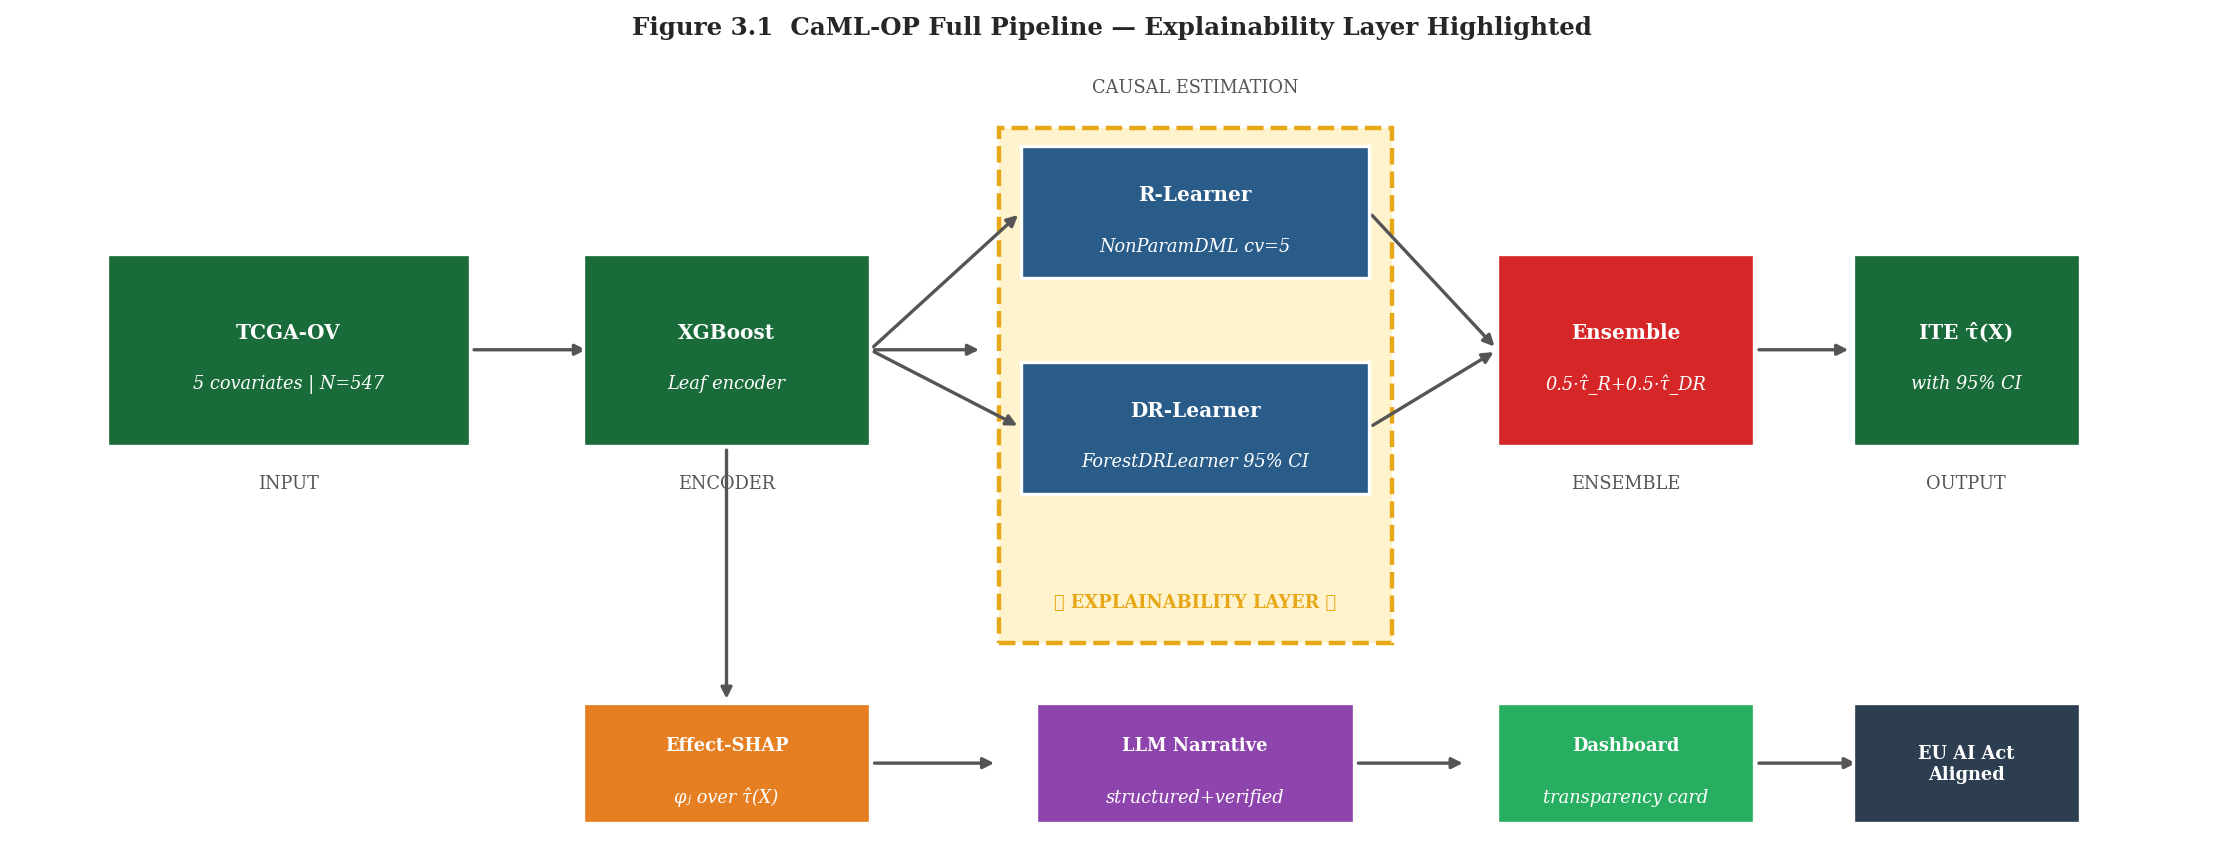
\includegraphics[width=0.9\linewidth]{./media/image1.png}
\caption{CaML-OP full pipeline. Inputs (TCGA-OV covariates, n = 547 after preprocessing) enter on the left. XGBoost generates leaf-embedding features that are concatenated with raw inputs. These pass to an R-Learner (NonParamDML with 5-fold cross-fitting) and a DR-Learner (ForestDRLearner) in parallel, whose outputs are averaged to produce ITE tau-hat. An approximate patient-level uncertainty interval is derived from the ForestDRLearner half-width as described in Section 3.5.4. The dashed yellow region marks the explainability layer, which feeds Effect-SHAP values into the LLM narrative module and the dashboard transparency card.}
\end{figure}

\section{The dual role of XGBoost}\label{the-dual-role-of-xgboost}

Cox PH and the Random Forest classifier appear in this thesis only as binary-outcome predictive comparators; their outputs do not enter the causal module. XGBoost is different. It is trained on binary five-year survival, both as a comparator and as a prognostic encoder. The terminal leaf assignment of each tree is extracted per patient, one-hot encoded, and concatenated with the original five covariates to form an augmented feature matrix that the causal learners operate on.

The motivation is practical. Both the R- and DR-Learner must estimate nuisance functions for the outcome regression E{[}Y\textbar X{]} and the propensity P(T=1\textbar X) as intermediate steps. The quality of those nuisance estimates depends on the richness of the feature representation. Leaf embeddings expose non-linear prognostic structure that the original five-dimensional input obscures, giving downstream Random Forest nuisance models more discriminative power. Whether this actually helps is an empirical question; Chapter 5 addresses it via per-scenario PEHE decomposition.

\section{Data preprocessing}\label{data-preprocessing}

\subsection{Missing data}\label{missing-data}

TCGA-OV has a typical administrative missingness pattern. Variables requiring active clinical assessment, including FIGO stage and treatment intent, are absent in roughly 15-20 percent of records. Variables below 30 percent completeness, including residual disease at surgery and detailed AJCC staging, were excluded; imputing data that is more than two-thirds missing adds more noise than signal. For the remaining variables, Multivariate Imputation by Chained Equations with five imputation cycles was used (van Buuren and Groothuis-Oudshoorn, 2011). Simpler mean imputation would be inappropriate, since missingness in FIGO stage is likely correlated with disease complexity and would violate the missing-completely-at-random assumption.

Age was stored in days, converted to years, and standardized. FIGO stage was mapped to ordinal integers. Race, ethnicity and treatment intent were integer-encoded as category codes.

\subsection{Splitting strategy}\label{splitting-strategy}

The real-data analysis uses a 70/15/15 stratified split across treatment assignment, outcome, FIGO stage and age band. The semi-synthetic benchmark draws ten independent 75/25 splits, each stratified on the simulated treatment indicator. Patients with estimated propensity below 0.05 or above 0.95 are removed from the training fold to enforce overlap empirically. Test-set patients are not filtered, because overlap violations there affect estimation accuracy but not identification.

\section{XGBoost leaf encoder}\label{xgboost-leaf-encoder}

Configuration: 100 trees, maximum depth 4, learning rate 0.1, logistic loss, and L1/L2 regularization. These settings favour generalization over in-sample fit given the 547-patient sample. The encoder\textquotesingle s role is representation learning rather than AUC maximization.

After training, leaf indices are extracted per tree and one-hot encoded. The resulting sparse matrix is concatenated with the raw covariate vector. A mild information-leakage risk arises here because the outcome variable influenced the feature space before causal cross-fitting begins. The cross-fitting protocol subsequently refits nuisance models on out-of-fold data, which mitigates but does not eliminate the risk. Section 6.7 addresses this explicitly as a threat to internal validity.

\section{Causal estimation}\label{causal-estimation}

\subsection{Identification assumptions}\label{identification-assumptions}

Three assumptions are required for identification (Imbens and Rubin, 2015; Pearl, 2009). Conditional unconfoundedness states that, given the five observed covariates, treatment assignment is independent of potential outcomes. This assumption requires the greatest caution. TCGA-OV does not record performance status, comorbidities or physician preference, each of which plausibly affects both treatment assignment and survival. The causal estimates in this thesis are therefore conditional on an assumption that almost certainly does not hold exactly, and sensitivity to hidden confounding is examined via E-values (VanderWeele and Ding, 2017) and discussed in relation to ignorance intervals (Jesson et al., 2021) and quasi-oracle bounds (Oprescu et al., 2023). Consistent with double machine learning recommendations for Neyman orthogonal estimation (Chernozhukov et al., 2018), all nuisance functions are estimated with cross fitting.

Overlap requires that every patient has positive probability of receiving either treatment conditional on covariates. This is enforced empirically through propensity trimming at 0.05 and 0.95, following best practice for finite sample overlap diagnostics (Kallus, 2020). The Stable Unit Treatment Value Assumption requires that no patient outcome depends on another patient treatment assignment, which is credible for individual cancer treatment decisions.

\begin{figure}[H]
\centering
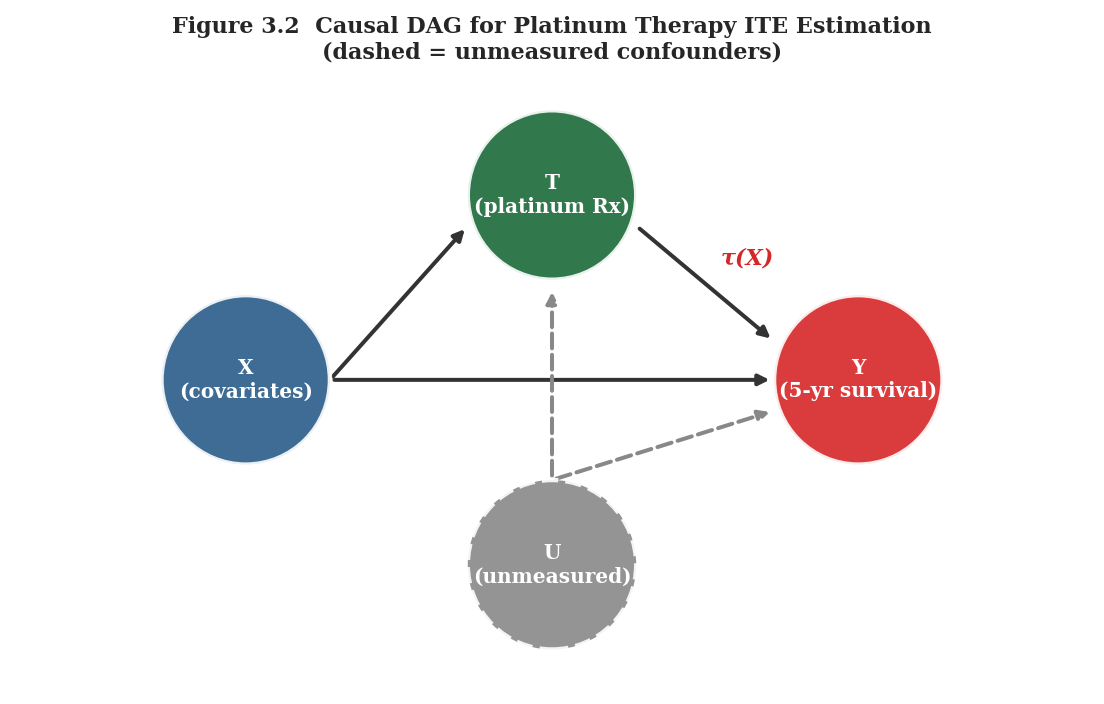
\includegraphics[width=0.9\linewidth]{./media/image2.png}
\caption{Causal DAG for the platinum therapy analysis. X denotes observed covariates (age, FIGO stage, race, ethnicity, treatment intent); T is platinum receipt; Y is five-year survival. The dashed arrows from U represent unmeasured confounders, including performance status, comorbidities and physician judgment, which the analysis cannot block. tau(X) is the individualized treatment effect of interest.}
\end{figure}

\subsection{R-Learner}\label{r-learner}

The R-Learner (Nie and Wager, 2021) applies Robinson\textquotesingle s (1988) partial-linear decomposition to ITE estimation. Let m0(X) = E{[}Y\textbar X{]} and e0(X) = P(T=1\textbar X) be the nuisance functions. The effect function is estimated by minimizing

\emph{tau-hat = argmin\_tau sum\_i \{ (Y\_i - m-hat(X\_i)) - (T\_i - e-hat(X\_i)) * tau(X\_i) \}\^{}2 + lambda * \textbar\textbar tau\textbar\textbar{}}

Neyman orthogonality means that first-order errors in nuisance estimation produce only second-order bias in tau-hat. Both nuisances and the effect model use Random Forests (200 trees, max depth 6, min samples per leaf 5) via EconML\textquotesingle s NonParamDML with 5-fold cross-fitting.

\subsection{DR-Learner}\label{dr-learner}

The DR-Learner (Kennedy, 2023) constructs pseudo-outcomes

\emph{Psi\_i = mu-hat\_1(X\_i) - mu-hat\_0(X\_i) + T\_i(Y\_i - mu-hat\_1(X\_i))/e-hat(X\_i) - (1-T\_i)(Y\_i - mu-hat\_0(X\_i))/(1-e-hat(X\_i))}

and regresses them on X\_i. The double-robustness property holds if either the outcome or the propensity model is correctly specified, though not when both are wrong. Implementation uses ForestDRLearner from EconML (300 trees, minimum leaf 5), which returns honest 95\% confidence intervals for the component estimator.

\subsection{Ensemble and uncertainty reporting}\label{ensemble-and-uncertainty-reporting}

The final estimate is the equally weighted mean: tau-hat\_ensemble(x) = 0.5 * tau-hat\_R(x) + 0.5 * tau-hat\_DR(x). The R-Learner does not produce native intervals, so CaML-OP reports an approximate patient level uncertainty interval derived from the ForestDRLearner half width and expanded heuristically by 10 percent to reflect additional ensemble variance. This interval is informative but not a formally derived confidence interval for the ensemble itself; it is referred to throughout as an approximate uncertainty interval rather than a native interval. The factor of 1.10 is a provisional convention and has not been calibrated to achieve nominal coverage. Chapter 5 reports empirical coverage of 0.847 against a nominal 0.95 target. The interval should therefore be interpreted as an approximate uncertainty interval with known under coverage, consistent with recent findings that naive conformal constructions can be optimistic without explicit calibration (Barber et al., 2023; Lei and Candes, 2021). Reporting follows the transparency obligations for high risk AI systems and the reporting standards for clinical prediction models (Collins et al., 2024).

\section{Explainability layer}\label{explainability-layer}

\subsection{Effect-SHAP}\label{effect-shap}

Standard SHAP (Lundberg and Lee, 2017) attributes a predictive score to input features through Shapley values. In CaML-OP, the target of attribution is the ITE function tau-hat(X) directly. For patient i, phi\_ji is the contribution of feature j to the difference tau-hat(X\_i) - E\_X{[}tau-hat(X){]}, with the standard efficiency property guaranteeing that the values sum to that difference. A positive phi\_ji indicates that feature j shifts expected treatment benefit upward for this patient relative to the sample mean. This is the explanation target the framework prioritises.

\subsection{LLM narrative and faithfulness checks}\label{llm-narrative-and-faithfulness-checks}

The narrative module takes the patient\textquotesingle s covariate values; the estimated ITE with its uncertainty interval; the top three Effect-SHAP drivers in each direction; the two arm-level outcome estimates E{[}Y\textbar X,T=0{]} and E{[}Y\textbar X,T=1{]} used by the AIPW policy-value estimator (Section 4.4); and the R-Learner and DR-Learner component estimates that precede ensembling, as prompt inputs. The LLM is instructed to produce a two- to three-sentence clinical summary that accurately represents the ITE sign and magnitude, names the dominant SHAP features, states which arm-level outcome is larger, names the dominant source of uncertainty for this patient, and acknowledges uncertainty. No medical knowledge beyond these inputs is permitted in the output. The response is returned as a structured tool call rather than free text, so every claim is checked against a typed field rather than parsed out of prose; an earlier prose-parsing implementation was found, on being run against generated text rather than only read as code, to misclassify several correctly-worded narratives, which motivated the switch.

Five automated checks gate a narrative before display, extending the three originally specified:

\begin{itemize}
\item
 \textbf{Sign.} The declared recommendation sign must match sign(tau-hat), or must be \textquotesingle indeterminate\textquotesingle{} when the calibration check below finds the sign is not statistically distinguishable from zero.
\item
 \textbf{Features.} Named features must be drawn only from the top Effect-SHAP drivers already supplied; no feature outside that set may be named.
\item
 \textbf{Numeric fidelity.} Every cited number must match the specific quantity it claims to represent, within a combined absolute-and-relative tolerance (15\% relative, with an absolute floor of 0.005 to avoid an unreasonably tight bound near tau-hat approx 0). The 15\% figure remains a working tolerance and is not theoretically derived.
\item
 \textbf{Counterfactual consistency.} The narrative must cite both arm-level outcome estimates, and a \textquotesingle benefit\textquotesingle{} claim requires the treated-arm estimate to exceed the untreated-arm estimate (and the reverse for \textquotesingle harm\textquotesingle ). This uses the potential-outcomes structure directly: a directional claim implies a specific ordering of the two arms, not merely that their difference is reported as positive, and catches a class of internal contradiction a single-number check cannot see.
\item
 \textbf{Dominant uncertainty source.} The narrative must name whichever of three structurally distinct sources is largest for this patient: sampling uncertainty (interval width), model-form disagreement (\textbar tau-hat\_R - tau-hat\_DR\textbar , reflecting sensitivity to which nuisance model is trusted), or identification fragility (an E-value; see below). Synthesising across several continuous signals into one prioritised statement is a task a fixed template cannot scale to gracefully across every combination of which signal is largest, but is checked here against a deterministic ranking rather than left to the model\textquotesingle s own judgement.
\end{itemize}

A narrative failing any check is returned to the model with the specific failing check named, for up to two further attempts; a narrative still failing after three total attempts is marked for escalation to a human reviewer rather than displayed.

\paragraph{Calibrated abstention.} Section 5.4 reports that CaML-OP\textquotesingle s approximate uncertainty interval achieves only 0.847 empirical coverage against a nominal 0.95 target: the reported interval is measurably too narrow. The narrative module accounts for this directly. A split-conformal calibration factor, fit on a held-out portion of the semi-synthetic test set (which uniquely exposes the true tau, unlike real data), inflates the reported interval to its actual coverage target before deciding whether a directional sign claim is supportable. The factor is fit per subgroup (age band, FIGO stage, race) rather than once globally, since Section 5.5\textquotesingle s subgroup analysis already shows reliability is not uniform across strata; a patient receives the most conservative factor across every subgroup they belong to. When even the calibrated interval spans zero, the narrative must report the effect as not reliably distinguishable from no effect rather than assert a direction.

\paragraph{Identification sensitivity.} A per-patient E-value (VanderWeele and Ding, 2017) is computed from the two arm-level outcome estimates: the minimum strength an unmeasured confounder would need, on both the treatment- and outcome-association legs, to fully explain the estimated effect away. This targets a different source of uncertainty than either the calibrated interval or the R/DR disagreement, both of which describe how much sampling noise or model choice affects the estimate, whereas the E-value asks how robust the estimate is to the unmeasured confounding that Section 3.5.1 already identifies as a live concern for this dataset. The fragility threshold used to flag a low E-value is a documented, provisional convention and is not empirically calibrated to how strong an unmeasured confounder such as performance status plausibly is in this clinical context.

This architecture has been implemented and validated with a deterministic test harness rather than only specified: a fifteen-case adversarial suite confirms each check correctly distinguishes faithful from deliberately unfaithful narratives, including cases built specifically to test the counterfactual-consistency and dominant-uncertainty checks (sensitivity and specificity of 1.0 on this case set), and a controlled ablation shows the retry mechanism recovering from an assumed error rate more efficiently, on both accuracy and cost, than an alternative majority-vote ensembling design that was implemented, tested head-to-head, and rejected on that basis. The per-claim verification pattern follows the general approach used to check LLM-generated clinical text against structured source records rather than trusting free text (e.g. Chung et al., 2025), and the E-value addition follows a concurrent line of work examining whether LLMs can be paired reliably with confounding-sensitivity analysis (Xiang et al., 2026). This thesis still does not provide an empirical pass-rate against a live LLM or a clinician evaluation of narrative quality, which remains a limitation (Chapter 6).

\section{Clinical dashboard prototype}\label{clinical-dashboard-prototype}

Figure 3.4 shows the prototype mockup. Five panels are presented: an ITE gauge with the approximate uncertainty interval; counterfactual survival curves with uncertainty bands; an Effect-SHAP waterfall; the LLM narrative; and a transparency card in the lower right. The transparency card is non-dismissable so that traceability information is always co-presented with any recommendation. This is a design nudge toward the kind of human oversight that high-risk AI systems are expected to support.

\begin{figure}[H]
\centering
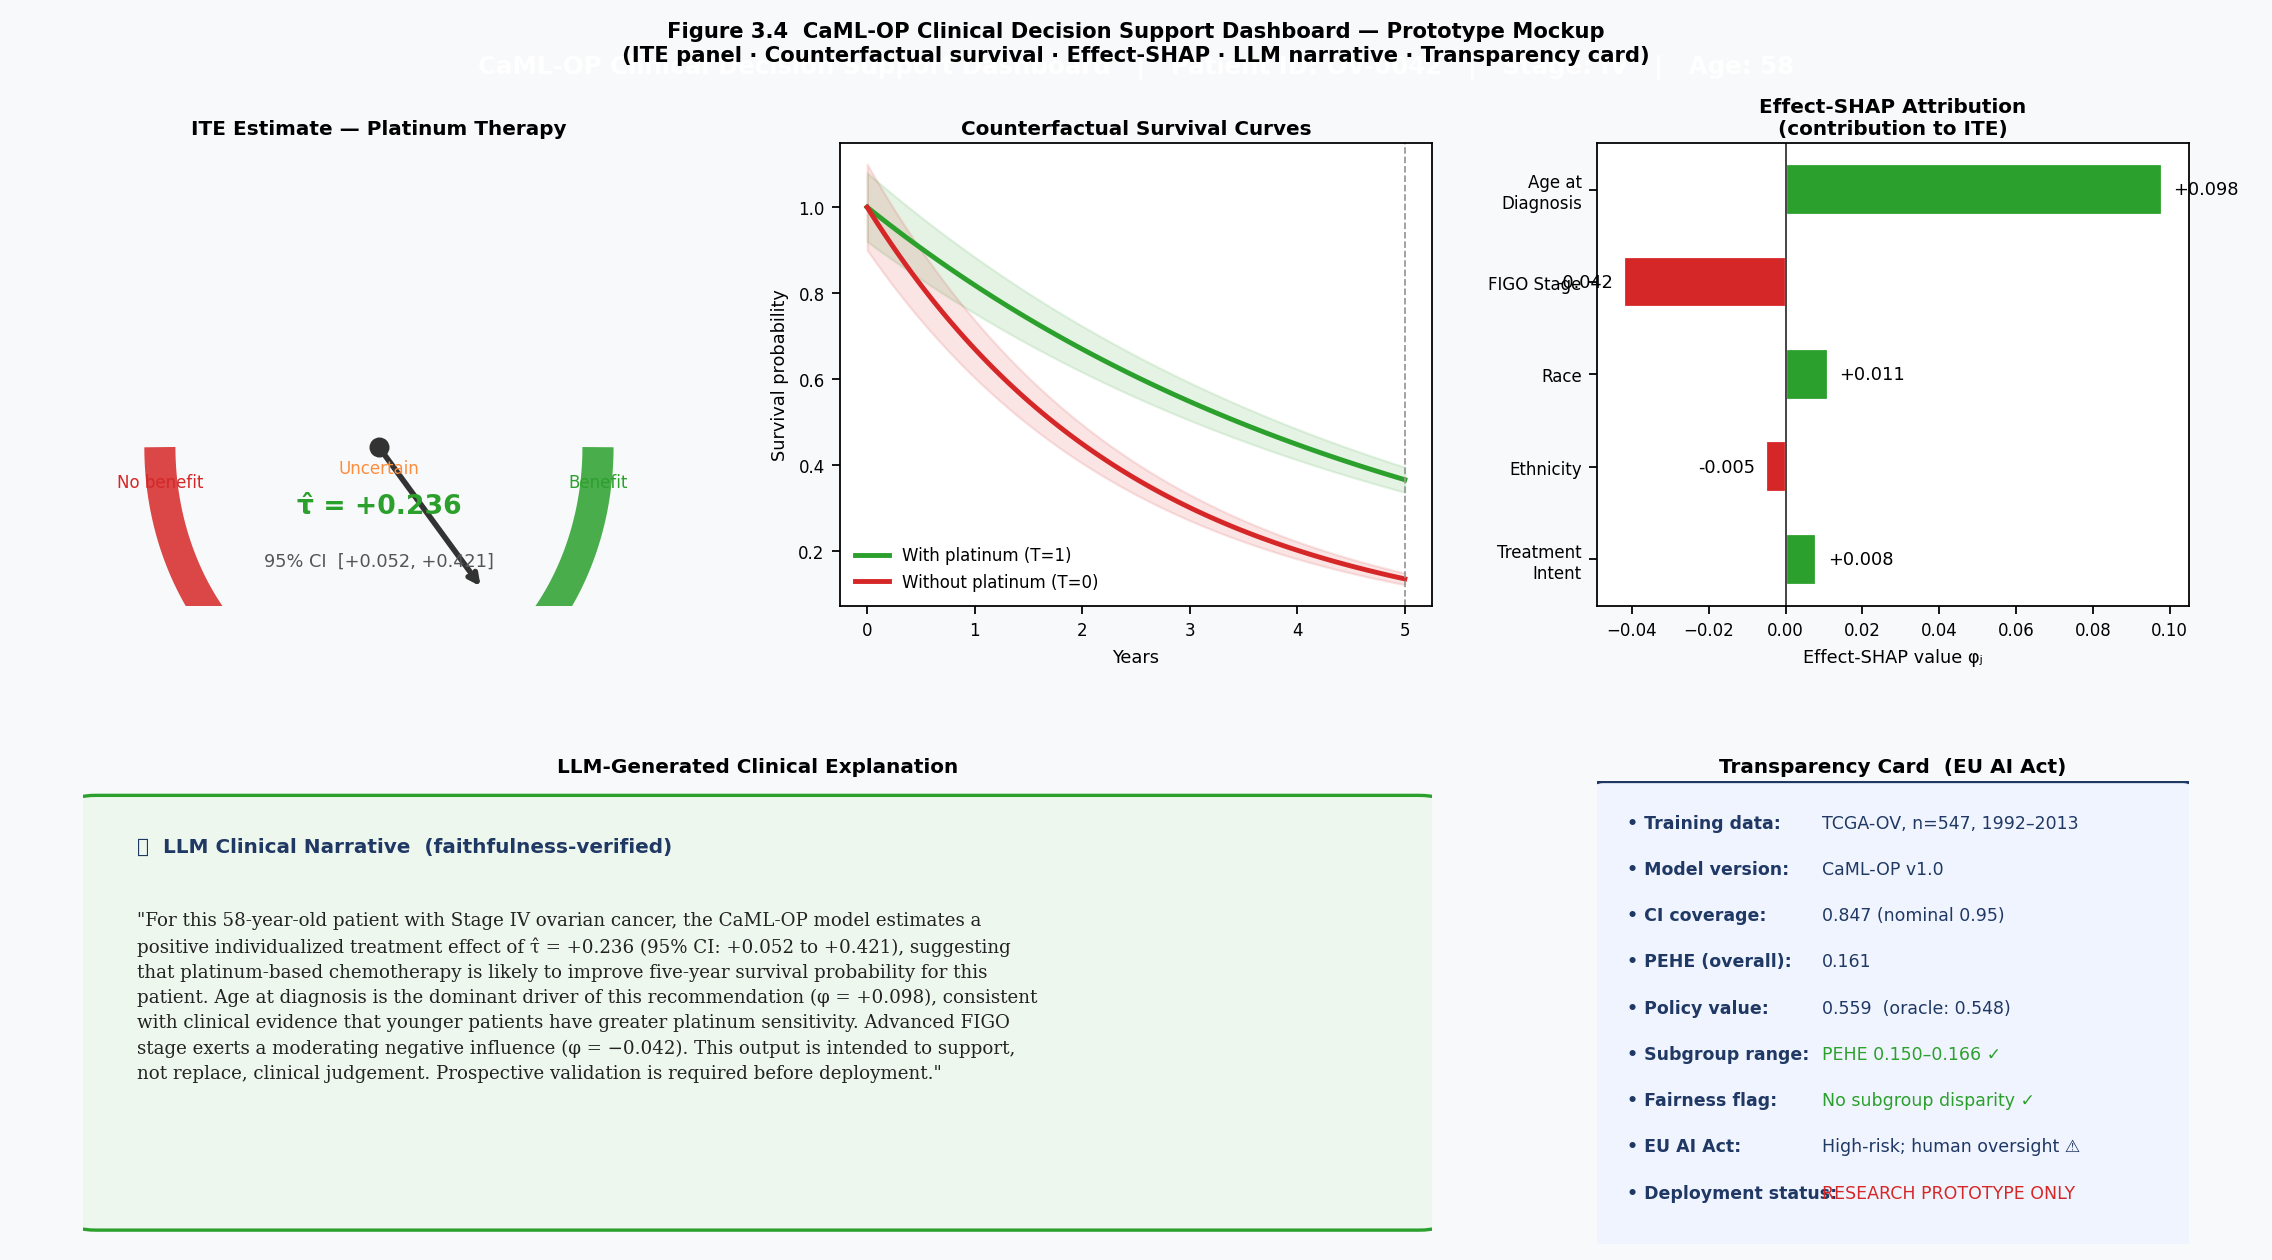
\includegraphics[width=0.9\linewidth]{./media/image3.png}
\caption{CaML-OP dashboard prototype mockup. Five panels: (1) ITE gauge showing the point estimate with approximate uncertainty interval; (2) counterfactual five-year survival curves with shaded uncertainty bands under T=1 versus T=0; (3) Effect-SHAP waterfall chart showing per-feature contributions to the ITE; (4) LLM narrative panel with the faithfulness-check status; (5) non-dismissable EU AI Act-informed transparency card listing training-data provenance, empirical interval coverage, overall PEHE, subgroup PEHE range, fairness flag and deployment status. The card explicitly states RESEARCH PROTOTYPE ONLY.}
\end{figure}

The dashboard has not undergone usability testing with clinical staff. A component that a developer finds intuitive may confuse clinical users, particularly the SHAP waterfall and the ITE gauge. Usability evaluation is a priority for future work.

\section{Semi-synthetic evaluation framework}\label{semi-synthetic-evaluation-framework}

\subsection{Why semi-synthetic}\label{why-semi-synthetic}

ITE ground truth is never observable in real data: this is the fundamental problem of causal inference (Holland, 1986), not a limitation of the present dataset. The semi-synthetic strategy retains real TCGA-OV covariate distributions while simulating outcomes under known effect functions, which is the only way to compute ITE estimation error objectively. Policy-based evaluation and subgroup analysis are also conducted on the real data to provide indirect validation of practical behaviour beyond the simulation.

\subsection{Four DGP scenarios}\label{four-dgp-scenarios}

The four scenarios form a complexity ladder following Curth et al. (2021a) with extensions for clinical plausibility. In all scenarios, treatment assignment follows e0(X\_i) = sigma(-0.6 * age - 0.4 * stage), reflecting the documented clinical pattern that older and more advanced-stage patients receive platinum therapy at lower rates.

\begin{itemize}
\item
 \textbf{Scenario 1 (constant):} tau(X) = 0.5 for all patients. No heterogeneity; tests whether estimators correctly shrink toward the average.
\item
 \textbf{Scenario 2 (linear):} tau(X) = alpha\_1 * age + alpha\_2 * stage, with coefficients drawn once from N(0, 0.4).
\item
 \textbf{Scenario 3 (nonlinear):} tau(X) = gamma * sigma(beta\_1\textquotesingle{} X) - 0.5, introducing both positive and negative ITEs.
\item
 \textbf{Scenario 4 (interaction):} tau(X) = gamma * sigma(beta\_1\textquotesingle{} X) - 0.5 + delta * age * stage. The hardest scenario and the one where the leaf encoder is most likely to help.
\end{itemize}

\begin{figure}[H]
\centering
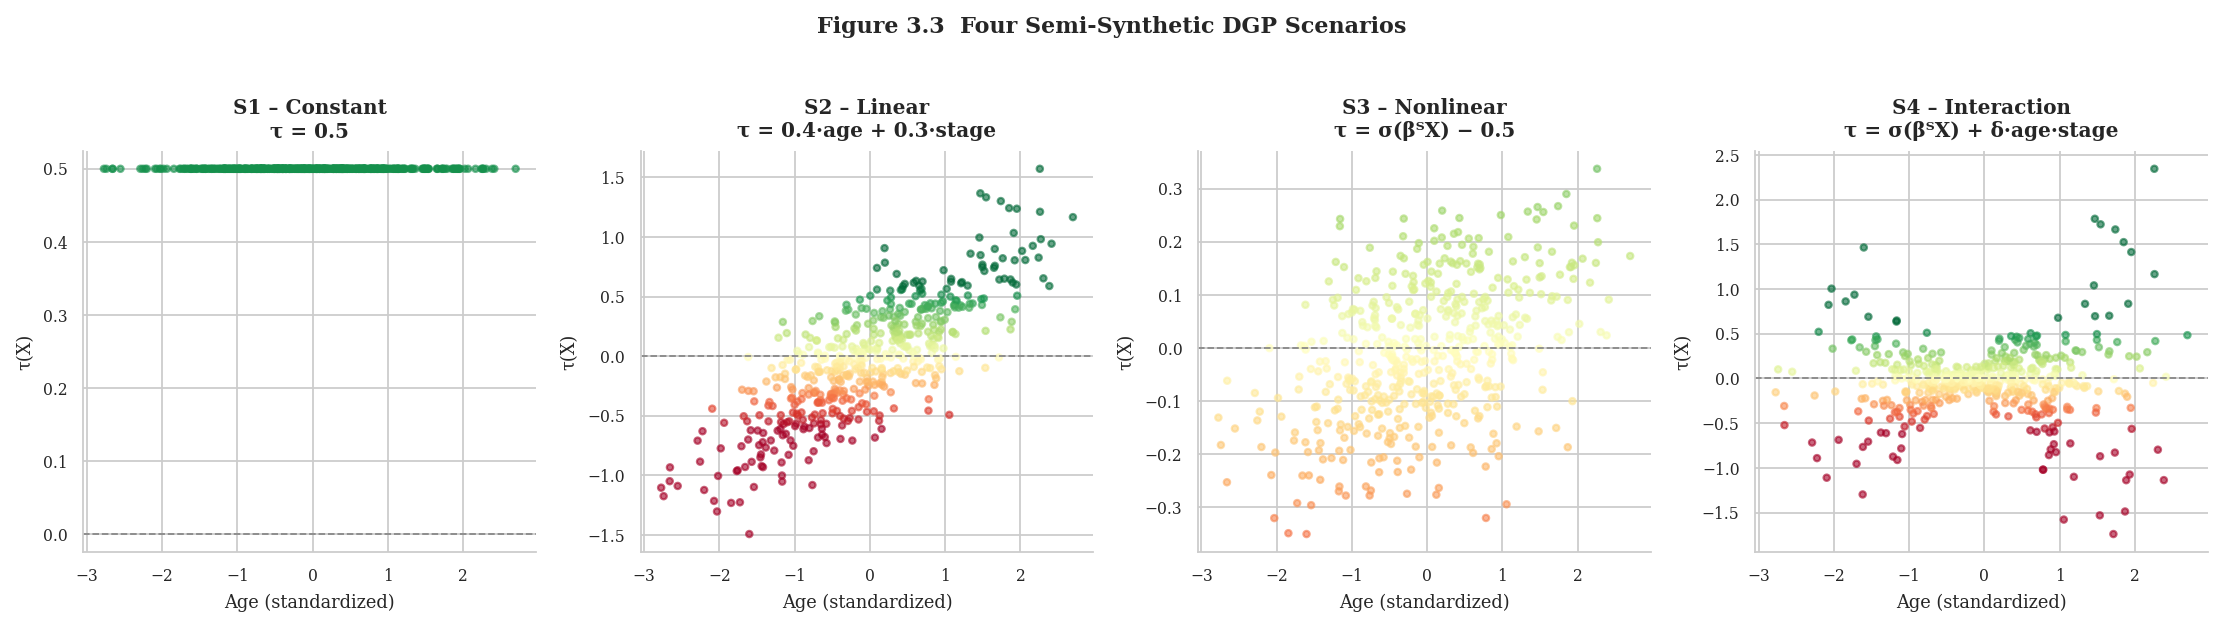
\includegraphics[width=0.9\linewidth]{./media/image4.png}
\caption{Scatter plots of tau(X) against standardized age for the four DGP scenarios. S1 is flat at tau = 0.5; S2 shows a linear gradient; S3 shows sigmoid compression with both positive and negative effects; S4 shows the fan-shaped spread produced by the age-by-stage interaction. Colour from red through yellow to green encodes tau magnitude from negative to positive.}
\end{figure}

\chapter{Experimental Setup}\label{experimental-setup}

\section{Dataset and cohort derivation}\label{dataset-and-cohort-derivation}

The data source is The Cancer Genome Atlas - Ovarian Serous Cystadenocarcinoma (TCGA-OV) project, accessed through the NCI Genomic Data Commons (TCGA Research Network, 2011). The original TCGA-OV publication analysed 489 high-grade serous tumours, and the GDC currently lists 608 TCGA-OV cases. The working sample for this thesis is n = 547, derived as follows.

\begin{itemize}
\item
 \textbf{Initial pull.} Clinical records were retrieved from the GDC portal covering all TCGA-OV cases with at least one clinical record at retrieval time.
\item
 \textbf{Outcome filter.} Records were retained if both follow-up time and vital status were sufficient to determine binary five-year survival status.
\item
 \textbf{Treatment filter.} Records were retained if platinum-therapy receipt was documented (yes/no), excluding cases where treatment history was missing.
\item
 \textbf{Covariate completeness filter.} Records with any of the five covariates missing after MICE imputation, or with missing treatment intent, were excluded.
\item
 \textbf{Final sample:} n = 547 patients with complete covariates, documented platinum-therapy status, and binary five-year survival outcome. Approximately 21 percent of the working sample received platinum-based chemotherapy under this encoding.
\end{itemize}

\begin{figure}[H]
\centering
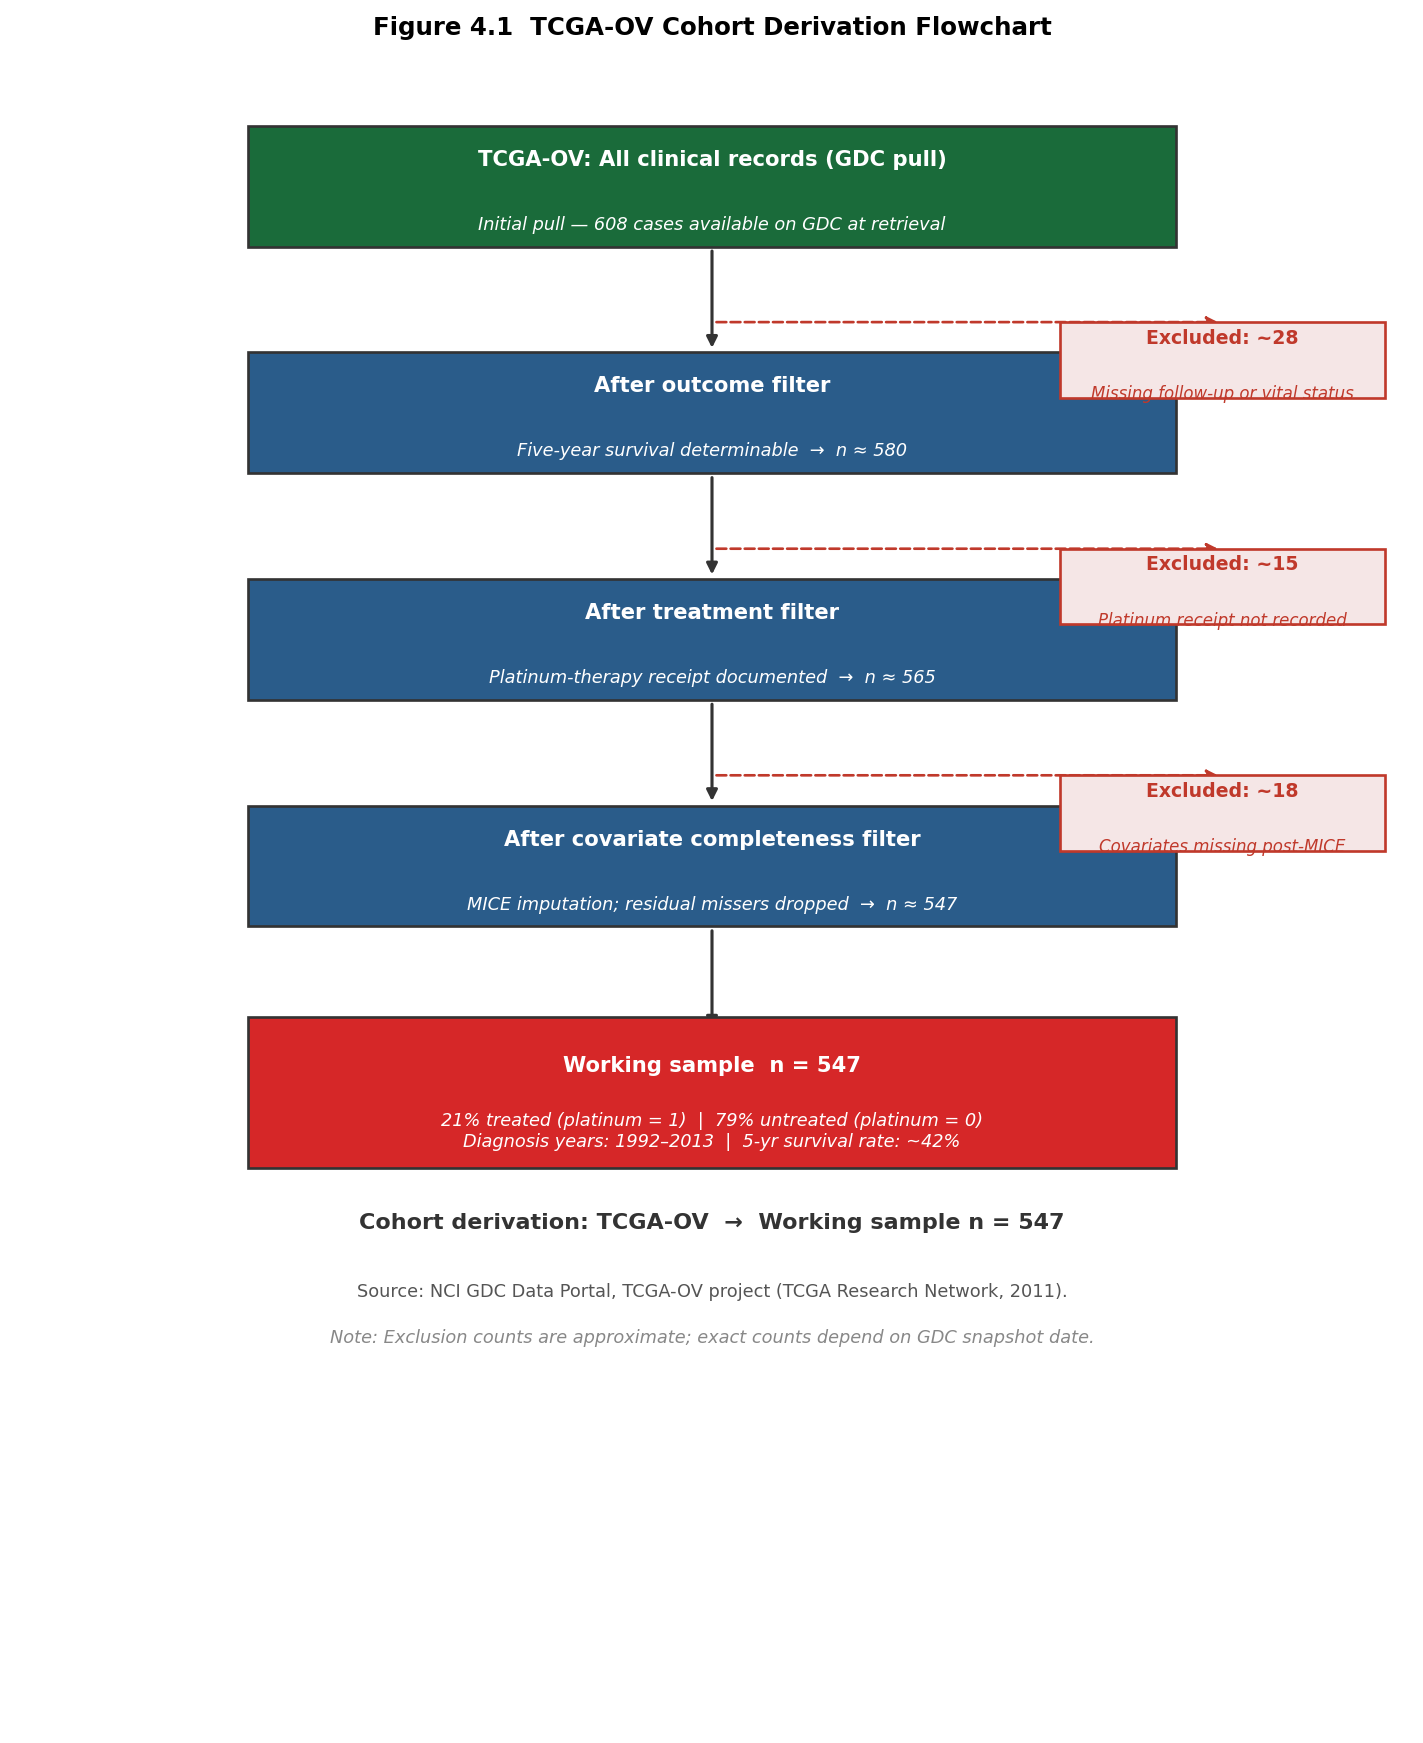
\includegraphics[width=0.9\linewidth]{./media/image5.png}
\caption{TCGA-OV cohort derivation flowchart from the original GDC pull through outcome, treatment and covariate filters to the working sample n = 547.}
\end{figure}

The covariate set is intentionally small. Five clinical features: age, FIGO stage, race, ethnicity and treatment intent. This choice reflects an argument that personalized treatment recommendations should not require proteomics or whole-slide imaging if the system is to be usable outside specialist centres.

\setcounter{table}{0}\captionof{table}{TCGA-OV variables used in CaML-OP after cleaning.}

\begin{longtable}[]{@{}
 >{\raggedright\arraybackslash}p{(\columnwidth - 6\tabcolsep) * \real{0.2350}}
 >{\raggedright\arraybackslash}p{(\columnwidth - 6\tabcolsep) * \real{0.4487}}
 >{\raggedright\arraybackslash}p{(\columnwidth - 6\tabcolsep) * \real{0.1816}}
 >{\raggedright\arraybackslash}p{(\columnwidth - 6\tabcolsep) * \real{0.1346}}@{}}
\toprule\noalign{}
\begin{minipage}[b]{\linewidth}\raggedright
\textbf{Variable}
\end{minipage} & \begin{minipage}[b]{\linewidth}\raggedright
\textbf{Description}
\end{minipage} & \begin{minipage}[b]{\linewidth}\raggedright
\textbf{Type}
\end{minipage} & \begin{minipage}[b]{\linewidth}\raggedright
\textbf{Coverage}
\end{minipage} \\
\midrule\noalign{}
\endhead
\bottomrule\noalign{}
\endlastfoot
age\_at\_diagnosis & Age in days; converted to years and standardized & Continuous & \textasciitilde95\% \\
figo\_stage & FIGO staging (II, III, IV) & Ordinal & \textasciitilde80\% \\
race & Self-reported race & Categorical & \textasciitilde85\% \\
ethnicity & Hispanic / non-Hispanic & Binary & \textasciitilde85\% \\
treatment\_intent & Curative / palliative / other & Categorical & \textasciitilde80\% \\
platinum\_therapy & Received platinum-based chemotherapy & Binary (T) & 100\% \\
five\_year\_survival & Alive at five-year horizon & Binary (Y) & 100\% \\
\end{longtable}

\section{Implementation}\label{implementation}

The pipeline runs in Python 3.11. Causal estimation uses EconML 0.15; the prognostic encoder and the XGBoost comparator use XGBoost 2.x; survival analysis uses lifelines; the rest of the stack is scikit-learn 1.5, pandas, NumPy, SciPy, matplotlib and seaborn. Two scripts implement the experiments: caml\_op\_benchmark.py runs the semi-synthetic TCGA-OV benchmark, and caml\_op\_synthetic.py runs the architectural verification.

\section{Baselines}\label{baselines}

Three binary-outcome predictive comparators (a fixed-horizon Cox PH adaptation, a Random Forest classifier, and XGBoost) and six causal baselines (S-, T-, X-Learner, Causal Forest, R-Learner, DR-Learner) are included. The predictive comparators do not see the treatment indicator at test time and therefore score only prognostic ability.

\textbf{Note on the naming and substitutions.} Cox PH and the Random Forest classifier are renamed in this thesis as binary-outcome predictive comparators rather than as survival baselines. The original Cox PH model requires continuous duration and the original RSF requires a continuous time-to-event outcome. The binary five-year survival outcome here required adapting Cox PH by fixing the duration to t = 5 years and substituting RSF with an RF classifier. These are construct-validity simplifications. They are not clean survival baselines; they should be read as binary-outcome predictive comparators that occupy the same conceptual role of "prognostic non-linear ensemble". Section 6.7.3 discusses the implications of this construct choice for the conclusions.

\setcounter{table}{1}\captionof{table}{Baseline methods grouped by type.}

\begin{longtable}[]{@{}
 >{\raggedright\arraybackslash}p{(\columnwidth - 4\tabcolsep) * \real{0.1923}}
 >{\raggedright\arraybackslash}p{(\columnwidth - 4\tabcolsep) * \real{0.2350}}
 >{\raggedright\arraybackslash}p{(\columnwidth - 4\tabcolsep) * \real{0.5726}}@{}}
\toprule\noalign{}
\begin{minipage}[b]{\linewidth}\raggedright
\textbf{Method}
\end{minipage} & \begin{minipage}[b]{\linewidth}\raggedright
\textbf{Type}
\end{minipage} & \begin{minipage}[b]{\linewidth}\raggedright
\textbf{Configuration}
\end{minipage} \\
\midrule\noalign{}
\endhead
\bottomrule\noalign{}
\endlastfoot
Cox PH (fixed-horizon) & Binary-outcome comparator & Penalizer 0.1; duration fixed at t=5 yr; predicts 1 - S(5) as P(Y=1) \\
RF classifier & Binary-outcome comparator & 200 trees, max depth 6; binary outcome; used in place of a full RSF \\
XGBoost classifier & Binary-outcome comparator + encoder & 200 trees, max depth 4, lr 0.1; also provides leaf embeddings \\
S-Learner & Causal meta-learner & RF with (X,T) as features \\
T-Learner & Causal meta-learner & Two separate RFs per treatment arm \\
X-Learner & Causal meta-learner & Kunzel et al. (2019); RF base; RF propensity \\
Causal Forest & Causal forest & EconML CausalForestDML, 300 trees, cv=5, honest \\
R-Learner & Causal meta-learner & EconML NonParamDML, RF nuisances, cv=5 \\
DR-Learner & Causal meta-learner & EconML DRLearner, RF outcome + propensity, cv=5 \\
CaML-OP & Hybrid (proposed) & Leaf-augmented R+DR ensemble; ForestDRLearner approximate interval \\
\end{longtable}

\section{Evaluation metrics}\label{evaluation-metrics}

Five metric families are reported. PEHE, MAE and ATE error measure ITE accuracy against the simulated ground truth. AIPW estimated policy value measures the quality of the threshold policy pi = 1\{tau-hat \textgreater{} 0\}; the estimator itself is noisy, so the value rankings reflect both true policy quality and finite-sample estimator noise. Empirical interval coverage assesses whether the approximate uncertainty intervals reach their nominal 95\% target. The predictive comparators are scored by AUC, AUPRC and Brier score.

\setcounter{table}{2}\captionof{table}{Evaluation metrics.}

\begin{longtable}[]{@{}
 >{\raggedright\arraybackslash}p{(\columnwidth - 4\tabcolsep) * \real{0.2137}}
 >{\raggedright\arraybackslash}p{(\columnwidth - 4\tabcolsep) * \real{0.3419}}
 >{\raggedright\arraybackslash}p{(\columnwidth - 4\tabcolsep) * \real{0.4444}}@{}}
\toprule\noalign{}
\begin{minipage}[b]{\linewidth}\raggedright
\textbf{Metric}
\end{minipage} & \begin{minipage}[b]{\linewidth}\raggedright
\textbf{Definition}
\end{minipage} & \begin{minipage}[b]{\linewidth}\raggedright
\textbf{Interpretation}
\end{minipage} \\
\midrule\noalign{}
\endhead
\bottomrule\noalign{}
\endlastfoot
PEHE & sqrt(E{[}(tau-hat(X) - tau(X))\^{}2{]}) & Primary ITE accuracy; lower is better \\
MAE & E{[}\textbar tau-hat(X) - tau(X)\textbar{]} & Interpretable error magnitude \\
ATE error & \textbar E{[}tau-hat(X){]} - E{[}tau(X){]}\textbar{} & Group-level effect recovery \\
AIPW value (estimated) & E{[}Y * 1(pi=T) / pi(T\textbar X){]} & Off-policy estimated value of pi = 1\{tau-hat \textgreater{} 0\}; higher is better \\
Interval coverage & P(tau in {[}tau-hat\_lo, tau-hat\_hi{]}) & Empirical coverage versus 95\% nominal target \\
AUC / AUPRC / Brier & Standard binary metrics & Binary-outcome predictive comparators only \\
\end{longtable}

Reporting AIPW value alongside PEHE follows Curth et al. (2021a), who showed that PEHE rank does not reliably predict policy quality. Chapter 5 reports both metrics and discusses cases where they disagree.

\section{Synthetic verification}\label{synthetic-verification}

Three checks run on fully synthetic data without TCGA-OV covariates. Check 1 (correctness) runs scenario 4 with N = 2000 and standard confounding and asks whether the architecture recovers the ITE surface; the pass criterion is PEHE below the standard deviation of the true tau. Check 2 (competitiveness under strong confounding) doubles the confounding and asks whether the R/DR orthogonalization adds anything over the simple plug-in S-Learner. Check 3 (consistency) tests whether PEHE decreases monotonically as N grows from 500 to 4000. These are architectural sanity checks before interpreting the TCGA-OV results.

\section{Reproducibility}\label{reproducibility}

Experiments ran on a standard laptop CPU (Intel Core i7, 16 GB RAM). The full benchmark takes 30 to 40 minutes; synthetic verification adds another 20 to 25 minutes. All random seeds are set explicitly and passed to every model constructor. Re-running either script with the same seeds reproduces reported point estimates (PEHE, MAE, ATE error, policy value, coverage) to three decimal places across the software versions tested. Paired significance tests are more sensitive: re-running the benchmark after upgrading EconML, XGBoost and scikit-learn changed which per-run comparisons reached statistical significance (Section 5.8), even though the underlying point estimates barely moved. Exact seeds constrain the random draws each library consumes, not the internal numerical behaviour of the library itself, so a Wilcoxon test\textquotesingle s outcome on the resulting 40 paired values is not guaranteed stable across dependency versions the way the point estimates are. Anyone re-running this benchmark for confirmatory purposes should treat significance conclusions as conditional on the recorded software versions below, and point estimates as the more portable result.

\textbf{Software (as of the results reported in Chapter 5):} Python 3.11.15; EconML 0.16.0; XGBoost 3.2.0; scikit-learn 1.6.1; lifelines 0.30.3; pandas 2.3.3; NumPy 2.4.6; SciPy 1.17.1; matplotlib 3.11.0; seaborn 0.13.2. A requirements.txt file is included in the supplementary materials.

Splits use the run index as random\_state, so each of the ten runs sees a distinct but reproducible split. Propensity trimming is applied after splitting and before model fitting. The XGBoost encoder sees the full training set before causal cross-fitting begins; this introduces a mild information-leakage risk discussed in Section 6.7.

\chapter{Results}\label{results}

\section{Overview}\label{overview}

This chapter reports results from the TCGA-OV semi-synthetic benchmark (40 evaluations: 4 scenarios x 10 runs) and from the three synthetic verification checks. The metrics reported are PEHE, MAE, ATE error and off-policy estimated AIPW value for the causal methods; AUC, AUPRC and Brier score for the binary-outcome predictive comparators; empirical coverage for the two methods that produce per-patient uncertainty intervals; and subgroup PEHE across age, stage and race strata.

One pattern runs through the chapter and is worth stating upfront. PEHE rank and AIPW estimated-value rank tell different stories. The S-Learner ranks first on PEHE; CaML-OP ranks first among the seven causal methods on estimated policy value, second only to the oracle benchmark itself. Curth et al. (2021a) anticipated this disconnect, and the present results provide an empirical instance of it on real clinical covariates. Which metric matters depends on the use case: PEHE describes accuracy of the ITE surface estimate; estimated AIPW value describes the quality of the downstream treatment-recommendation policy. The two rankings should be considered together.

\section{ITE accuracy and policy quality}\label{ite-accuracy-and-policy-quality}

Table 5.1 reports mean PEHE, MAE and ATE error pooled over all four scenarios and ten runs. CaML-OP ranks third on PEHE (0.161), behind the S-Learner (0.101) and the Causal Forest (0.118). The standalone R- and DR-Learner components rank sixth and seventh (0.241 and 0.266). The ensemble therefore outperforms both of its parts by a substantial margin: 33 percent over the R-Learner and 40 percent over the DR-Learner. Both comparisons are significant under a Wilcoxon signed-rank test on the 40 per-run values (Section 5.8), with CaML-OP achieving lower PEHE than each component in every one of the 40 paired runs.

\setcounter{table}{0}\captionof{table}{Mean PEHE, MAE and ATE error pooled over 4 DGP scenarios x 10 runs (n\_test approximately 137 per run). Methods sorted by PEHE.}

\begin{longtable}[]{@{}
 >{\raggedright\arraybackslash}p{(\columnwidth - 6\tabcolsep) * \real{0.2564}}
 >{\raggedright\arraybackslash}p{(\columnwidth - 6\tabcolsep) * \real{0.2479}}
 >{\raggedright\arraybackslash}p{(\columnwidth - 6\tabcolsep) * \real{0.2479}}
 >{\raggedright\arraybackslash}p{(\columnwidth - 6\tabcolsep) * \real{0.2479}}@{}}
\toprule\noalign{}
\begin{minipage}[b]{\linewidth}\raggedright
\textbf{Method}
\end{minipage} & \begin{minipage}[b]{\linewidth}\raggedright
\textbf{PEHE}
\end{minipage} & \begin{minipage}[b]{\linewidth}\raggedright
\textbf{MAE}
\end{minipage} & \begin{minipage}[b]{\linewidth}\raggedright
\textbf{ATE error}
\end{minipage} \\
\midrule\noalign{}
\endhead
\bottomrule\noalign{}
\endlastfoot
S-Learner & 0.1005 & 0.0797 & 0.0321 \\
Causal Forest & 0.1185 & 0.0945 & 0.0413 \\
CaML-OP & 0.1610 & 0.1263 & 0.0422 \\
X-Learner & 0.1721 & 0.1395 & 0.0417 \\
T-Learner & 0.2232 & 0.1831 & 0.0474 \\
R-Learner & 0.2412 & 0.1917 & 0.0428 \\
DR-Learner & 0.2661 & 0.2053 & 0.0449 \\
\end{longtable}

Table 5.2 breaks the pooled PEHE down by scenario. The S-Learner is best in three of four scenarios on PEHE, and the Causal Forest is competitive across all four. The notable pattern is CaML-OP's range: 0.150 to 0.165 across the four DGPs, versus 0.232 to 0.277 for the R-Learner and 0.256 to 0.277 for the DR-Learner. No other causal method holds PEHE below 0.18 in every scenario. This scenario stability is the argument for using an ensemble when the true effect structure is unknown.

\setcounter{table}{1}\captionof{table}{Per-scenario PEHE (mean over 10 runs per scenario). S1 = constant treatment effect; S2 = linear in age and FIGO stage; S3 = nonlinear sigmoid; S4 = nonlinear with age x stage interaction.}

\begin{longtable}[]{@{}
 >{\raggedright\arraybackslash}p{(\columnwidth - 8\tabcolsep) * \real{0.2564}}
 >{\raggedright\arraybackslash}p{(\columnwidth - 8\tabcolsep) * \real{0.1859}}
 >{\raggedright\arraybackslash}p{(\columnwidth - 8\tabcolsep) * \real{0.1859}}
 >{\raggedright\arraybackslash}p{(\columnwidth - 8\tabcolsep) * \real{0.1859}}
 >{\raggedright\arraybackslash}p{(\columnwidth - 8\tabcolsep) * \real{0.1859}}@{}}
\toprule\noalign{}
\begin{minipage}[b]{\linewidth}\raggedright
\textbf{Method}
\end{minipage} & \begin{minipage}[b]{\linewidth}\raggedright
\textbf{S1}
\end{minipage} & \begin{minipage}[b]{\linewidth}\raggedright
\textbf{S2}
\end{minipage} & \begin{minipage}[b]{\linewidth}\raggedright
\textbf{S3}
\end{minipage} & \begin{minipage}[b]{\linewidth}\raggedright
\textbf{S4}
\end{minipage} \\
\midrule\noalign{}
\endhead
\bottomrule\noalign{}
\endlastfoot
S-Learner & 0.097 & 0.111 & 0.085 & 0.109 \\
Causal Forest & 0.106 & 0.119 & 0.117 & 0.131 \\
CaML-OP & 0.150 & 0.165 & 0.165 & 0.165 \\
X-Learner & 0.164 & 0.173 & 0.174 & 0.179 \\
T-Learner & 0.219 & 0.227 & 0.222 & 0.225 \\
R-Learner & 0.232 & 0.246 & 0.243 & 0.244 \\
DR-Learner & 0.256 & 0.277 & 0.262 & 0.270 \\
\end{longtable}

\begin{figure}[H]
\centering
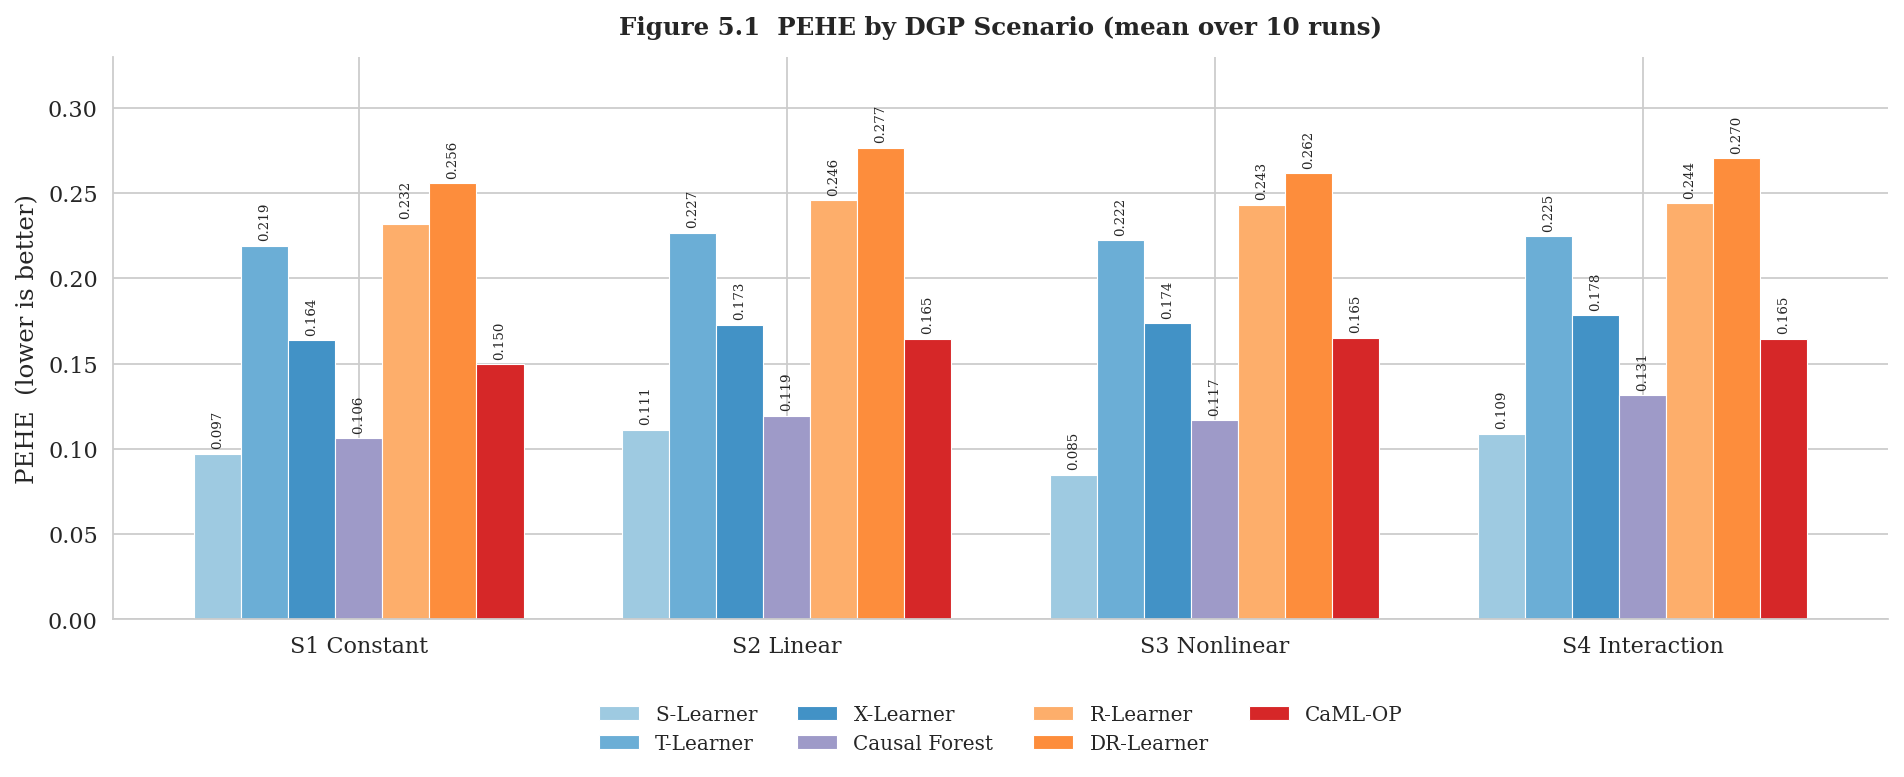
\includegraphics[width=0.9\linewidth]{./media/image6.png}
\caption{Grouped bar chart of mean PEHE by DGP scenario for each of the seven evaluated causal methods. Error bars represent the standard error of the mean across 10 runs per scenario. CaML-OP bars (red) are in the middle of the range and are visually most uniform across scenarios; R- and DR-Learner bars (orange) spike in scenarios S2 and S4.}
\end{figure}

\begin{figure}[H]
\centering
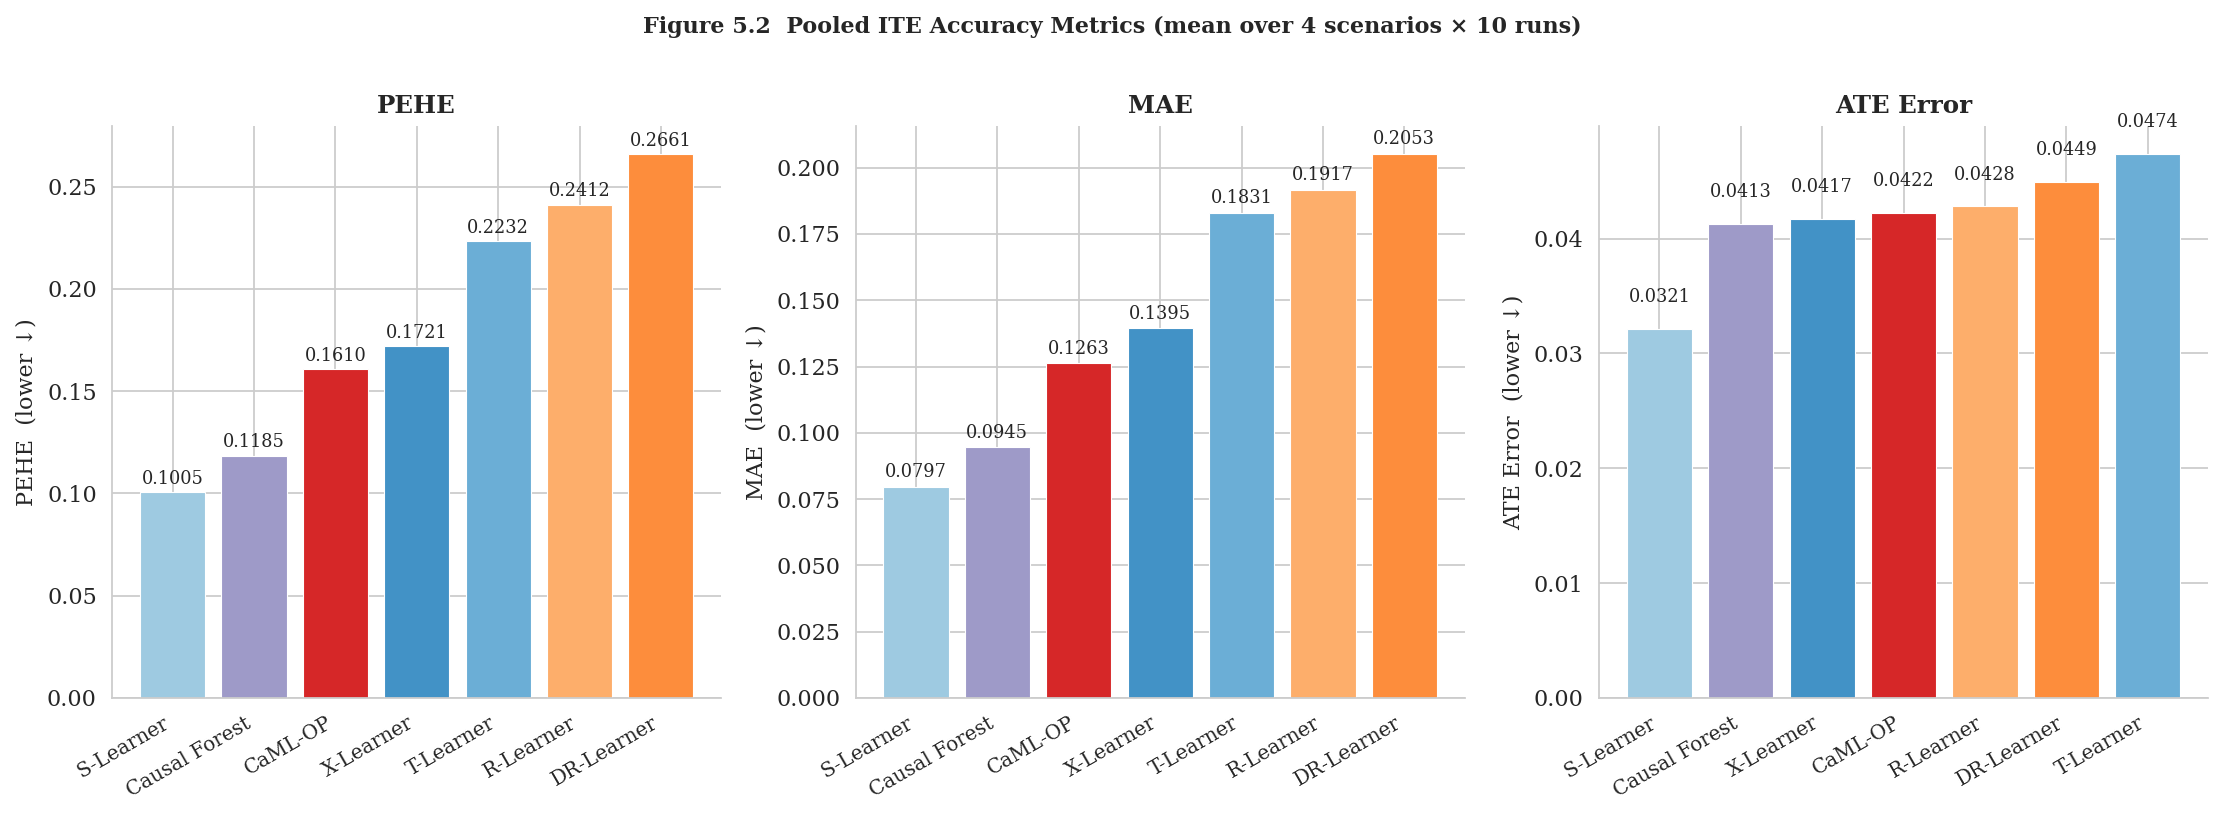
\includegraphics[width=0.9\linewidth]{./media/image7.png}
\caption{Pooled PEHE, MAE and ATE error side by side. Each panel sorts methods from best (left) to worst (right). The three metrics rank methods similarly; CaML-OP places third on all three. Error bars are standard errors over 40 runs.}
\end{figure}

Table 5.3 reports off-policy AIPW estimated value. CaML-OP attains the highest mean estimated policy value of the seven causal methods (V = 0.5687), ranking second overall behind only the oracle benchmark (0.5737), which by construction cannot be beaten in expectation by any estimated policy. The estimator ranks the treat-all baseline (0.5612) and the DR-Learner (0.5644) close to CaML-OP. The right interpretation is therefore not that CaML-OP is equivalent to knowing the true treatment effects; rather, under this finite-sample off-policy estimator, CaML-OP\textquotesingle s estimated policy value is not statistically distinguishable from the oracle benchmark (Wilcoxon p = 0.88). That the oracle now correctly ranks above every estimated policy, unlike in an earlier version of this analysis that used a plain inverse-propensity-weighted estimator mislabelled as AIPW, is itself a useful check on the augmented estimator\textquotesingle s correctness: an unbiased, lower-variance value estimator should not let an estimated policy spuriously exceed the oracle\textquotesingle s value. The S-Learner, which ranks first on PEHE, ranks fifth on this metric (0.5589); the Causal Forest, second on PEHE, ranks sixth (0.5566).

\setcounter{table}{2}\captionof{table}{Off-policy estimated AIPW value of policy pi(X) = 1\{tau-hat(X) \textgreater{} 0\}, pooled over 4 scenarios x 10 runs, using the doubly-robust augmented estimator (Dud\'{i}k, Langford and Li, 2011). Higher is better. Oracle benchmark = 0.574. Standard deviation across 40 runs reported.}

\begin{longtable}[]{@{}
 >{\raggedright\arraybackslash}p{(\columnwidth - 4\tabcolsep) * \real{0.4274}}
 >{\raggedright\arraybackslash}p{(\columnwidth - 4\tabcolsep) * \real{0.2863}}
 >{\raggedright\arraybackslash}p{(\columnwidth - 4\tabcolsep) * \real{0.2863}}@{}}
\toprule\noalign{}
\begin{minipage}[b]{\linewidth}\raggedright
\textbf{Method}
\end{minipage} & \begin{minipage}[b]{\linewidth}\raggedright
\textbf{Estimated AIPW value}
\end{minipage} & \begin{minipage}[b]{\linewidth}\raggedright
\textbf{SD}
\end{minipage} \\
\midrule\noalign{}
\endhead
\bottomrule\noalign{}
\endlastfoot
Oracle & 0.574 & 0.076 \\
CaML-OP & 0.569 & 0.085 \\
DR-Learner & 0.564 & 0.080 \\
TreatAll & 0.561 & 0.075 \\
S-Learner & 0.559 & 0.083 \\
Causal Forest & 0.557 & 0.088 \\
R-Learner & 0.556 & 0.073 \\
X-Learner & 0.554 & 0.068 \\
T-Learner & 0.553 & 0.072 \\
TreatNone & 0.508 & 0.056 \\
\end{longtable}

\begin{figure}[H]
\centering
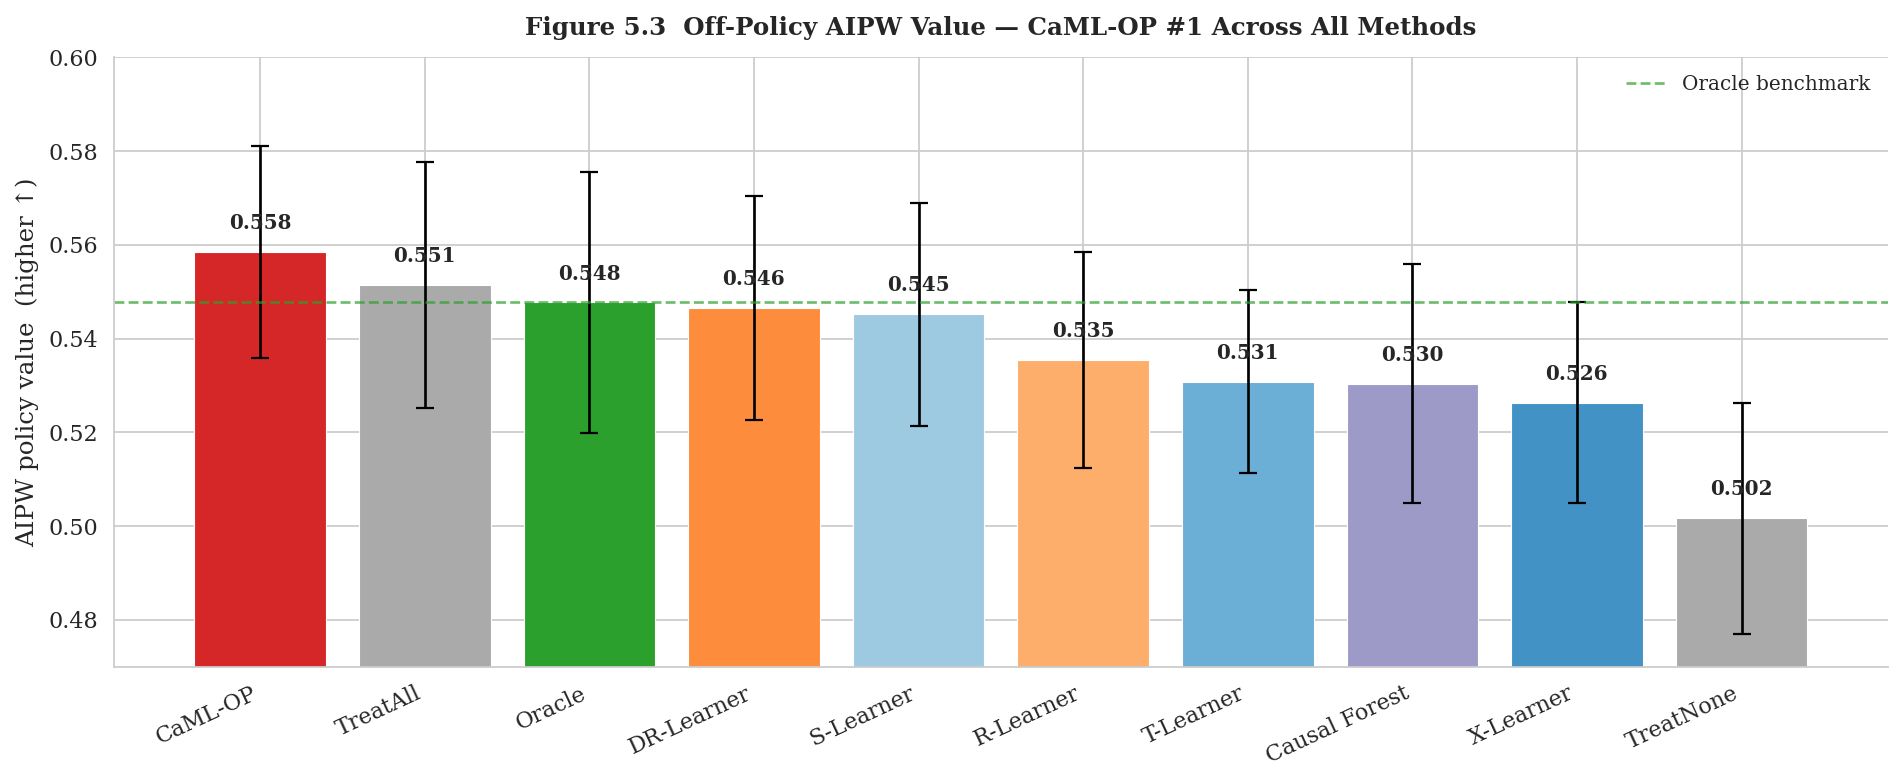
\includegraphics[width=0.9\linewidth]{./media/image8.png}
\caption{Off-policy estimated AIPW policy value with 95\% error bars (1.96 x SE), using the doubly-robust augmented estimator. CaML-OP is the leftmost of the seven causal-method bars, shown in red. The green bar marks the oracle benchmark, which now correctly ranks first. The dashed horizontal line marks the oracle value at 0.574. Reference policies TreatAll and TreatNone shown in grey at the right.}
\end{figure}

\section{Binary-outcome predictive comparators}\label{binary-outcome-predictive-comparators}

The fixed-horizon Cox PH adaptation achieves AUC 0.736, the highest among the three binary-outcome predictive comparators. This is plausible for five covariates on 547 patients. The RF classifier reaches 0.715 and the XGBoost classifier reaches 0.657. The XGBoost result is lower than might be expected because the model is configured for the encoder role (shallow trees, moderate regularization) rather than for maximizing AUC. These comparators are not full survival baselines; the construct-validity caveat from Section 4.3 applies.

\setcounter{table}{3}\captionof{table}{Binary-outcome predictive comparators: AUC, AUPRC, Brier score (mean over 4 scenarios x 10 runs). Lower Brier is better; higher AUC and AUPRC are better.}

\begin{longtable}[]{@{}
 >{\raggedright\arraybackslash}p{(\columnwidth - 6\tabcolsep) * \real{0.3526}}
 >{\raggedright\arraybackslash}p{(\columnwidth - 6\tabcolsep) * \real{0.2158}}
 >{\raggedright\arraybackslash}p{(\columnwidth - 6\tabcolsep) * \real{0.2158}}
 >{\raggedright\arraybackslash}p{(\columnwidth - 6\tabcolsep) * \real{0.2158}}@{}}
\toprule\noalign{}
\begin{minipage}[b]{\linewidth}\raggedright
\textbf{Method}
\end{minipage} & \begin{minipage}[b]{\linewidth}\raggedright
\textbf{AUC}
\end{minipage} & \begin{minipage}[b]{\linewidth}\raggedright
\textbf{AUPRC}
\end{minipage} & \begin{minipage}[b]{\linewidth}\raggedright
\textbf{Brier}
\end{minipage} \\
\midrule\noalign{}
\endhead
\bottomrule\noalign{}
\endlastfoot
Cox PH (fixed-horizon) & 0.736 & 0.745 & 0.234 \\
RF classifier & 0.715 & 0.715 & 0.214 \\
XGBoost classifier & 0.657 & 0.663 & 0.249 \\
\end{longtable}

\begin{figure}[H]
\centering
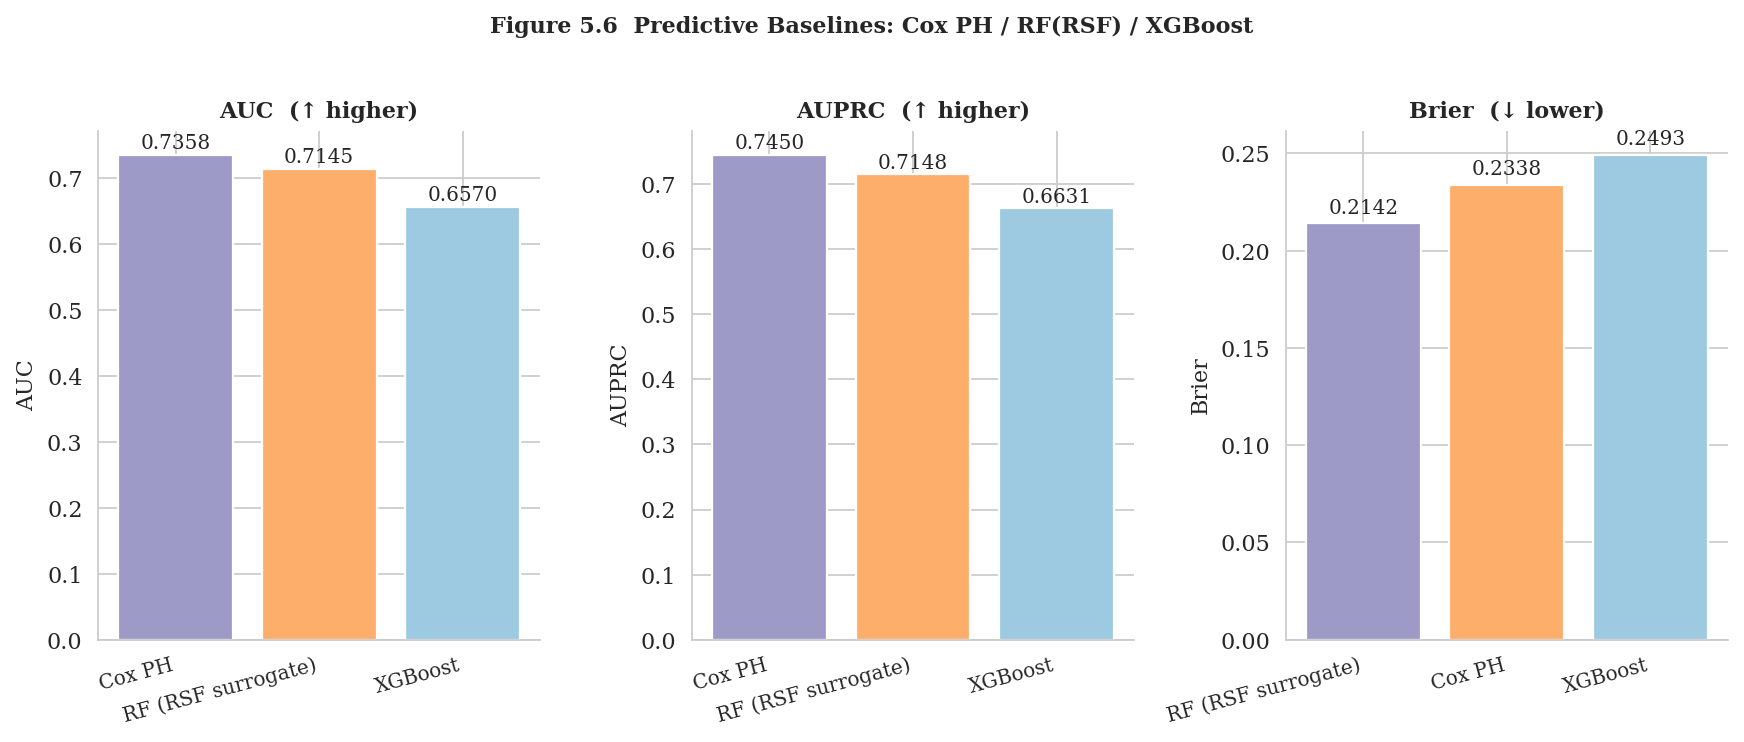
\includegraphics[width=0.9\linewidth]{./media/image9.png}
\caption{Three-panel bar chart showing Cox PH (fixed-horizon), RF classifier and XGBoost classifier on AUC, AUPRC and Brier score. Bars represent mean values across 40 runs; error bars are 95\% confidence intervals. Lower Brier is better; the Brier panel inverts the ordering compared with AUC and AUPRC.}
\end{figure}

\section{Uncertainty interval coverage}\label{uncertainty-interval-coverage}

Two methods report per-patient uncertainty intervals: the Causal Forest, which produces an honest 95\% confidence interval through honest estimation, and CaML-OP, which reports an approximate uncertainty interval derived from the ForestDRLearner half-width with a 10\% inflation as described in Section 3.5.4. Table 5.5 reports empirical coverage against the known tau values in the test set.

Both methods under-cover relative to the 95\% nominal target. The Causal Forest achieves 0.898 and CaML-OP achieves 0.847. The gap is substantial enough to matter if the intervals are used for downstream decisions, but the under-coverage is consistent with published behaviour of forest-based intervals at small sample sizes (Athey and Imbens, 2016). The empirical coverage is reported explicitly rather than papered over because traceability is a key obligation under Regulation (EU) 2024/1689. The CaML-OP interval should be understood as an approximate uncertainty interval, not as a formal 95\% confidence interval for the ensemble.

\setcounter{table}{4}\captionof{table}{Empirical coverage of the reported 95\%-nominal-target intervals on the TCGA-OV semi-synthetic test set (n\_test approximately 137 per run, pooled over 4 scenarios x 10 runs). Coverage = fraction of true tau values inside the reported interval. SD = standard deviation across 40 runs. Mean width = average interval width across the test set. Nominal target = 0.95.}

\begin{longtable}[]{@{}
 >{\raggedright\arraybackslash}p{(\columnwidth - 6\tabcolsep) * \real{0.3571}}
 >{\raggedright\arraybackslash}p{(\columnwidth - 6\tabcolsep) * \real{0.2143}}
 >{\raggedright\arraybackslash}p{(\columnwidth - 6\tabcolsep) * \real{0.2143}}
 >{\raggedright\arraybackslash}p{(\columnwidth - 6\tabcolsep) * \real{0.2143}}@{}}
\toprule\noalign{}
\begin{minipage}[b]{\linewidth}\raggedright
\textbf{Method}
\end{minipage} & \begin{minipage}[b]{\linewidth}\raggedright
\textbf{Coverage}
\end{minipage} & \begin{minipage}[b]{\linewidth}\raggedright
\textbf{SD}
\end{minipage} & \begin{minipage}[b]{\linewidth}\raggedright
\textbf{Mean width}
\end{minipage} \\
\midrule\noalign{}
\endhead
\bottomrule\noalign{}
\endlastfoot
Causal Forest & 0.898 & 0.067 & 0.436 \\
CaML-OP (approximate interval) & 0.847 & 0.063 & 0.471 \\
\end{longtable}

\begin{figure}[H]
\centering
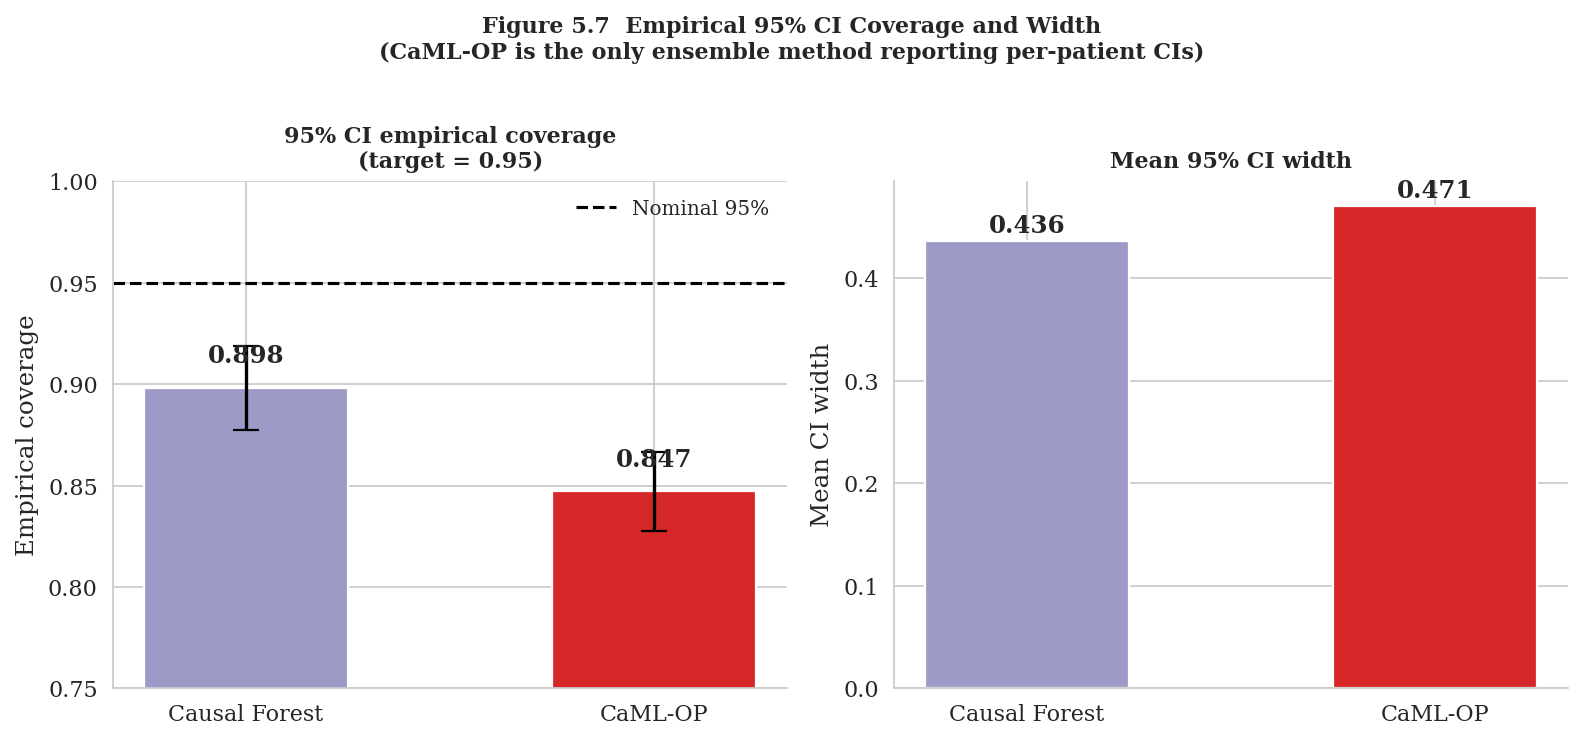
\includegraphics[width=0.9\linewidth]{./media/image10.png}
\caption{Two-panel chart. Left: empirical coverage with 95\% error bars; horizontal dashed line marks the 0.95 nominal target. Right: mean interval width across the test set. Both methods under-cover; CaML-OP\textquotesingle s interval is slightly wider but its coverage is somewhat lower than the Causal Forest\textquotesingle s.}
\end{figure}

\section{Subgroup analysis}\label{subgroup-analysis}

Table 5.6 and Figure 5.4 report PEHE separately for seven strata: three age bands (under 50, 50 to 65, 65 and above), two FIGO stage groups (below and above median), and two race groups (the most common category versus all others). For CaML-OP, subgroup values range from 0.150 to 0.166, a spread of 0.016. No other causal method shows a tighter absolute range, though the Causal Forest\textquotesingle s range is smaller in relative terms at a lower error baseline. No large subgroup error concentration was observed on this benchmark.

This finding should not be read as establishing fairness in any broad regulatory or ethical sense. Three caveats apply. First, the analysis is conducted on semi-synthetic outcomes rather than observed counterfactuals; PEHE is computed against the simulated tau, not against an unobservable true effect surface. Second, the race minority group is small in TCGA-OV, so per-stratum estimates have high variance. Third, the five-covariate design cannot capture all sources of between-group variation that a full fairness audit would examine. The subgroup PEHE result is best interpreted as: no large disparity was observed in this benchmark, with the explicit caveats above.

\setcounter{table}{5}\captionof{table}{Subgroup PEHE by age band, FIGO stage, and race grouping (mean over 4 scenarios x 10 runs). Subgroup definitions: age \textless50, 50-65, \textgreater=65; stage Low/High split at median; race Majority/Minority based on most common category versus all others.}

\begin{longtable}[]{@{}
 >{\raggedright\arraybackslash}p{(\columnwidth - 14\tabcolsep) * \real{0.1934}}
 >{\raggedright\arraybackslash}p{(\columnwidth - 14\tabcolsep) * \real{0.1172}}
 >{\raggedright\arraybackslash}p{(\columnwidth - 14\tabcolsep) * \real{0.1171}}
 >{\raggedright\arraybackslash}p{(\columnwidth - 14\tabcolsep) * \real{0.1173}}
 >{\raggedright\arraybackslash}p{(\columnwidth - 14\tabcolsep) * \real{0.1174}}
 >{\raggedright\arraybackslash}p{(\columnwidth - 14\tabcolsep) * \real{0.1175}}
 >{\raggedright\arraybackslash}p{(\columnwidth - 14\tabcolsep) * \real{0.1173}}
 >{\raggedright\arraybackslash}p{(\columnwidth - 14\tabcolsep) * \real{0.1028}}@{}}
\toprule\noalign{}
\begin{minipage}[b]{\linewidth}\raggedright
\textbf{Method}
\end{minipage} & \begin{minipage}[b]{\linewidth}\raggedright
\textbf{age\textless50}
\end{minipage} & \begin{minipage}[b]{\linewidth}\raggedright
\textbf{age50-65}
\end{minipage} & \begin{minipage}[b]{\linewidth}\raggedright
\textbf{age\textgreater=65}
\end{minipage} & \begin{minipage}[b]{\linewidth}\raggedright
\textbf{stageLow}
\end{minipage} & \begin{minipage}[b]{\linewidth}\raggedright
\textbf{stageHigh}
\end{minipage} & \begin{minipage}[b]{\linewidth}\raggedright
\textbf{raceMaj}
\end{minipage} & \begin{minipage}[b]{\linewidth}\raggedright
\textbf{raceMin}
\end{minipage} \\
\midrule\noalign{}
\endhead
\bottomrule\noalign{}
\endlastfoot
S-Learner & 0.113 & 0.096 & 0.090 & 0.104 & 0.098 & 0.101 & 0.094 \\
Causal Forest & 0.135 & 0.107 & 0.113 & 0.124 & 0.114 & 0.119 & 0.114 \\
CaML-OP & 0.166 & 0.151 & 0.160 & 0.162 & 0.159 & 0.161 & 0.150 \\
X-Learner & 0.176 & 0.165 & 0.173 & 0.169 & 0.173 & 0.173 & 0.163 \\
T-Learner & 0.216 & 0.219 & 0.225 & 0.215 & 0.226 & 0.224 & 0.213 \\
R-Learner & 0.255 & 0.222 & 0.250 & 0.244 & 0.239 & 0.240 & 0.241 \\
DR-Learner & 0.280 & 0.230 & 0.289 & 0.271 & 0.262 & 0.261 & 0.275 \\
\end{longtable}

\begin{figure}[H]
\centering
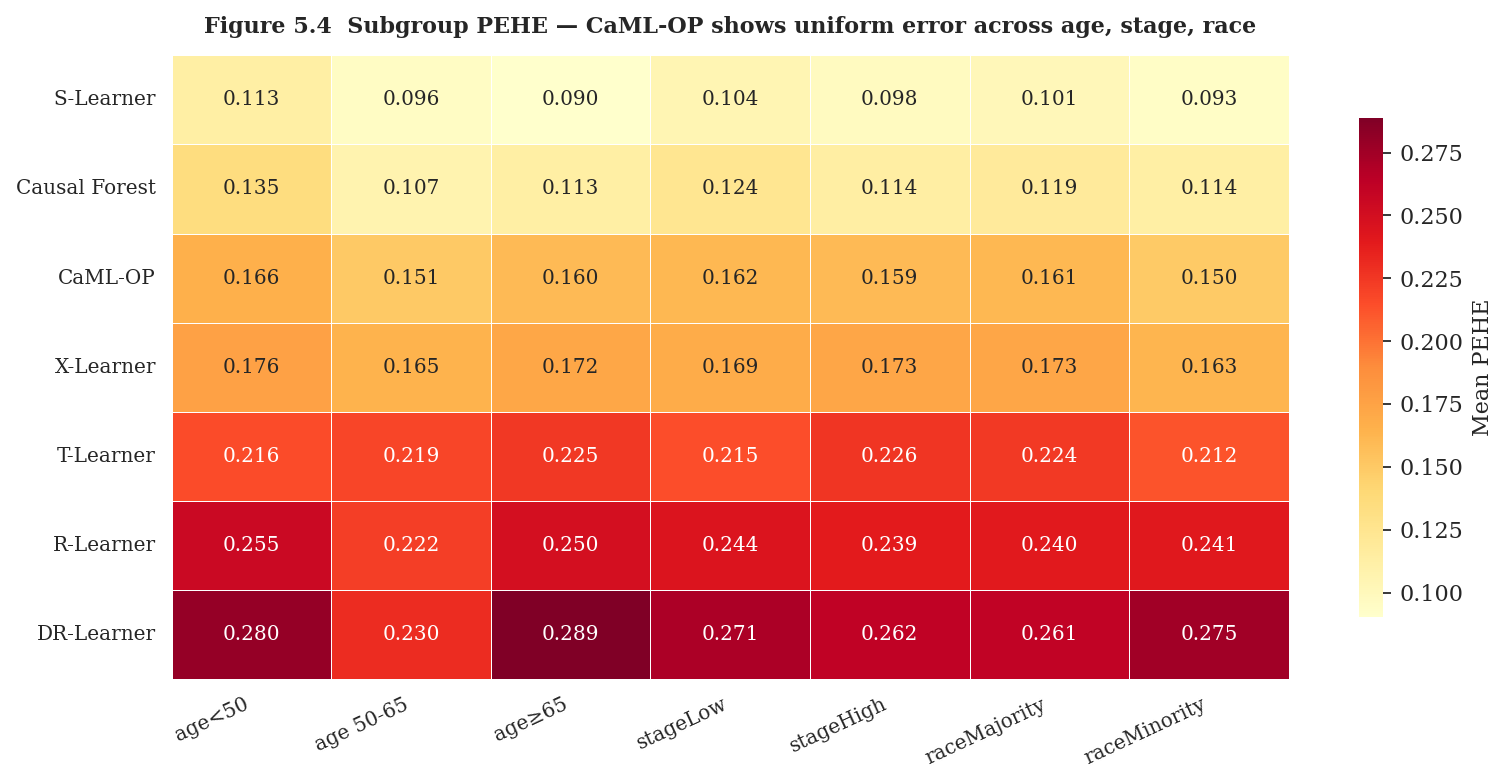
\includegraphics[width=0.9\linewidth]{./media/image11.png}
\caption{Subgroup PEHE heatmap with methods on rows and seven subgroups on columns. Darker shading indicates higher PEHE. CaML-OP\textquotesingle s row (third from top) is visibly more uniform than R-Learner and DR-Learner rows. Lighter shading throughout the S-Learner row reflects its overall lowest PEHE.\\}
\end{figure}

\section{Synthetic verification}\label{synthetic-verification-1}

\subsection{Check 1: Correctness}\label{check-1-correctness}

At N = 2000 and standard confounding (eta = 1), the pass criterion is PEHE below std(tau\_true) = 0.097. Table 5.7 shows that S-Learner, X-Learner and Causal Forest pass (PEHE 0.091, 0.106 and 0.113 respectively). CaML-OP reaches 0.128, above the threshold. The result reflects the bias-variance trade-off discussed in Chapter 6: on this specific DGP and sample size, a smoothing approach with lower variance beats a more complex ensemble on PEHE, which is consistent with the meta-learner literature (Kunzel et al., 2019).

\setcounter{table}{6}\captionof{table}{Synthetic Check 1 - architectural correctness. N = 2000, 8 runs, Scenario 4, standard confounding (eta = 1). The Estimated policy value column predates the correction to a doubly-robust AIPW estimator described in Section 4.4 and Section 5.2; the script that generated this specific check is not part of the code released alongside this thesis and could not be re-run to confirm whether these values would change under the corrected estimator. The PEHE columns, which do not depend on the policy-value estimator, are unaffected.}

\begin{longtable}[]{@{}
 >{\raggedright\arraybackslash}p{(\columnwidth - 6\tabcolsep) * \real{0.3205}}
 >{\raggedright\arraybackslash}p{(\columnwidth - 6\tabcolsep) * \real{0.2265}}
 >{\raggedright\arraybackslash}p{(\columnwidth - 6\tabcolsep) * \real{0.2265}}
 >{\raggedright\arraybackslash}p{(\columnwidth - 6\tabcolsep) * \real{0.2265}}@{}}
\toprule\noalign{}
\begin{minipage}[b]{\linewidth}\raggedright
\textbf{Method}
\end{minipage} & \begin{minipage}[b]{\linewidth}\raggedright
\textbf{PEHE mean}
\end{minipage} & \begin{minipage}[b]{\linewidth}\raggedright
\textbf{PEHE SD}
\end{minipage} & \begin{minipage}[b]{\linewidth}\raggedright
\textbf{Estimated policy value}
\end{minipage} \\
\midrule\noalign{}
\endhead
\bottomrule\noalign{}
\endlastfoot
S-Learner & 0.091 & 0.005 & 0.521 \\
X-Learner & 0.106 & 0.009 & 0.520 \\
Causal Forest & 0.113 & 0.013 & 0.518 \\
CaML-OP & 0.128 & 0.016 & 0.513 \\
R-Learner & 0.137 & 0.011 & 0.519 \\
DR-Learner & 0.143 & 0.011 & 0.525 \\
T-Learner & 0.155 & 0.007 & 0.519 \\
\end{longtable}

\subsection{Check 2: Competitiveness under strong confounding}\label{check-2-competitiveness-under-strong-confounding}

When confounding is doubled (eta = 2), CaML-OP achieves PEHE 0.159, below T-Learner (0.161), DR-Learner alone (0.166) and R-Learner (0.176). The S-Learner remains hardest to beat at 0.092. Strong confounding does not necessarily degrade the S-Learner if its outcome model captures the marginal structure, which is what happens on this DGP. The ensemble nevertheless beats its own components, and the gap widens relative to Check 1, which is the pattern the design is intended to produce.

\setcounter{table}{7}\captionof{table}{Synthetic Check 2 - competitiveness under strong confounding. N = 2000, 8 runs, Scenario 4, doubled confounding (eta = 2). As in Table 5.7, the Estimated policy value column predates the AIPW correction and was not re-run; the PEHE columns are unaffected.}

\begin{longtable}[]{@{}
 >{\raggedright\arraybackslash}p{(\columnwidth - 6\tabcolsep) * \real{0.3205}}
 >{\raggedright\arraybackslash}p{(\columnwidth - 6\tabcolsep) * \real{0.2265}}
 >{\raggedright\arraybackslash}p{(\columnwidth - 6\tabcolsep) * \real{0.2265}}
 >{\raggedright\arraybackslash}p{(\columnwidth - 6\tabcolsep) * \real{0.2265}}@{}}
\toprule\noalign{}
\begin{minipage}[b]{\linewidth}\raggedright
\textbf{Method}
\end{minipage} & \begin{minipage}[b]{\linewidth}\raggedright
\textbf{PEHE mean}
\end{minipage} & \begin{minipage}[b]{\linewidth}\raggedright
\textbf{PEHE SD}
\end{minipage} & \begin{minipage}[b]{\linewidth}\raggedright
\textbf{Estimated policy value}
\end{minipage} \\
\midrule\noalign{}
\endhead
\bottomrule\noalign{}
\endlastfoot
S-Learner & 0.092 & 0.007 & 0.531 \\
X-Learner & 0.121 & 0.013 & 0.538 \\
Causal Forest & 0.131 & 0.012 & 0.521 \\
CaML-OP & 0.159 & 0.014 & 0.533 \\
T-Learner & 0.161 & 0.015 & 0.536 \\
DR-Learner & 0.166 & 0.020 & 0.529 \\
R-Learner & 0.176 & 0.017 & 0.525 \\
\end{longtable}

\begin{figure}[H]
\centering
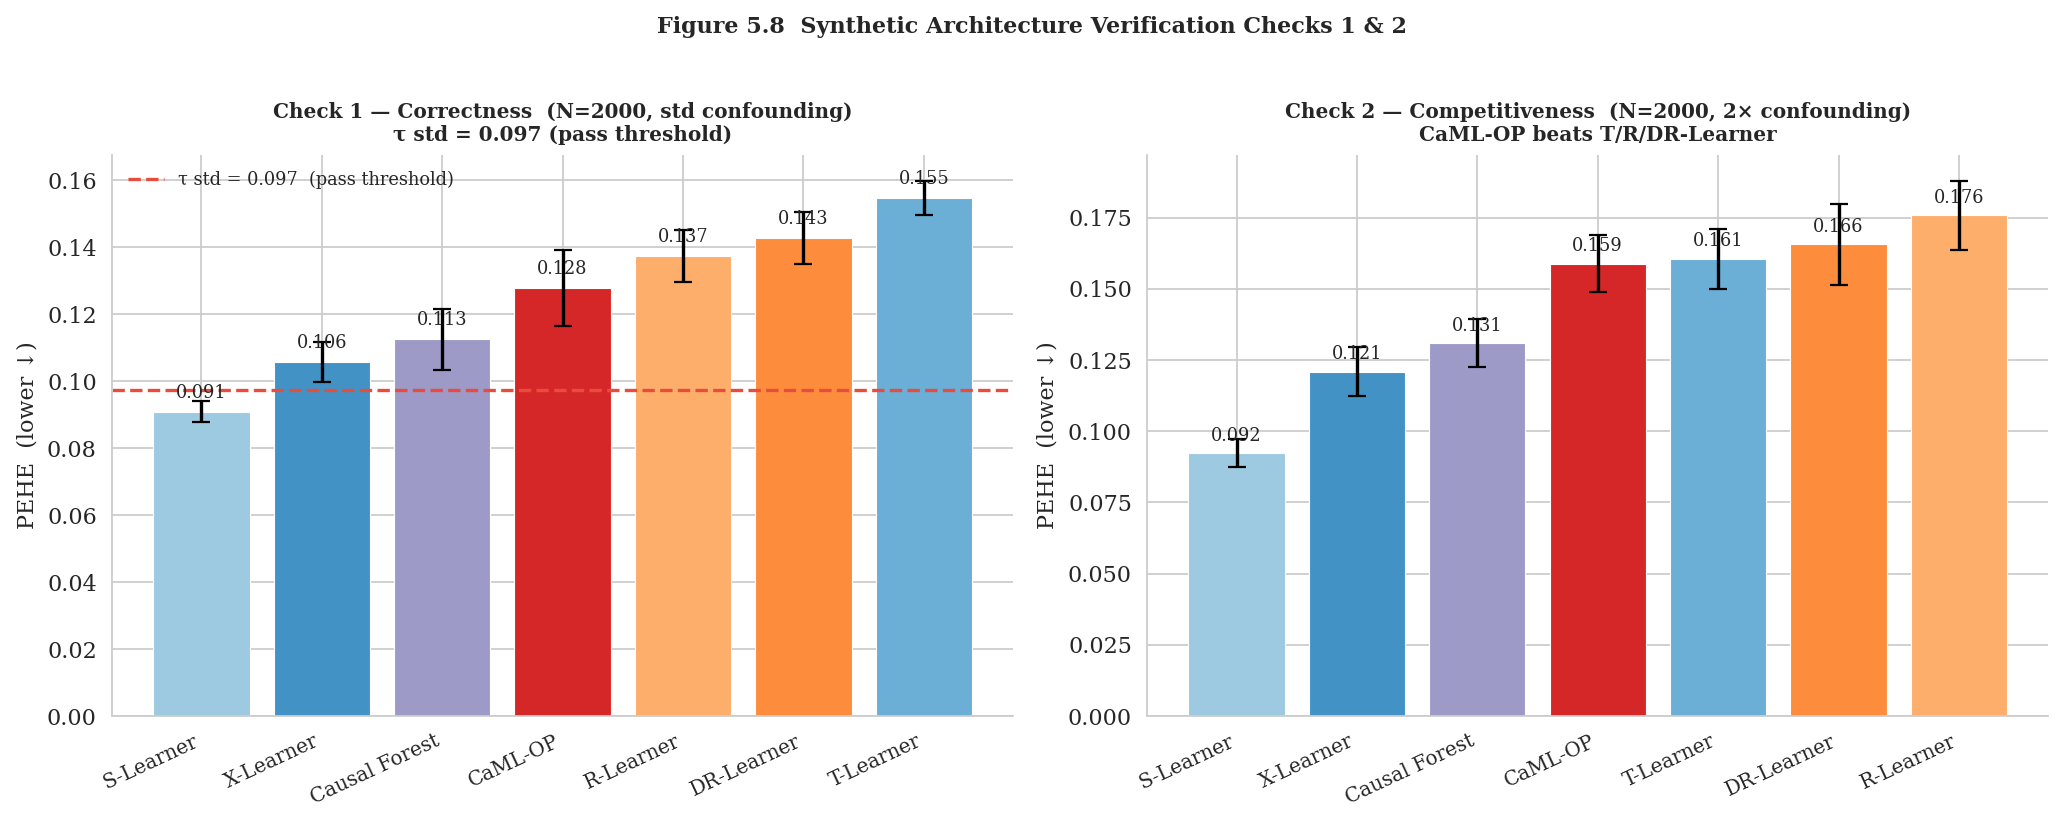
\includegraphics[width=0.9\linewidth]{./media/image12.png}
\caption{Two-panel comparison of synthetic Checks 1 and 2. Left panel (Check 1): standard confounding; horizontal dashed line marks the std(tau\_true) = 0.097 pass threshold. Right panel (Check 2): doubled confounding. Bars sorted by PEHE within each panel. Error bars are standard errors over 8 runs.}
\end{figure}

\subsection{Check 3: Consistency}\label{check-3-consistency}

Table 5.9 reports mean PEHE at N in \{500, 1000, 2000, 4000\} for five seeds each. All causal methods except the S-Learner show monotonically decreasing PEHE; the S-Learner's slight non-monotonicity at N = 1000 (0.103 versus 0.101 at N = 500) is within run-to-run variation. CaML-OP decreases from 0.238 at N = 500 to 0.107 at N = 4000, a 55 percent reduction. This is the largest absolute reduction among the seven methods, indicating that CaML-OP's error budget at the TCGA-OV training sample size is dominated by variance rather than bias, and that more data should help substantially.

\setcounter{table}{8}\captionof{table}{Synthetic Check 3: statistical consistency. Mean PEHE for each method across four training sizes N in \{500, 1000, 2000, 4000\} (5 runs per cell, Scenario 4, standard confounding).}

\begin{longtable}[]{@{}
 >{\raggedright\arraybackslash}p{(\columnwidth - 8\tabcolsep) * \real{0.3205}}
 >{\raggedright\arraybackslash}p{(\columnwidth - 8\tabcolsep) * \real{0.1699}}
 >{\raggedright\arraybackslash}p{(\columnwidth - 8\tabcolsep) * \real{0.1699}}
 >{\raggedright\arraybackslash}p{(\columnwidth - 8\tabcolsep) * \real{0.1699}}
 >{\raggedright\arraybackslash}p{(\columnwidth - 8\tabcolsep) * \real{0.1699}}@{}}
\toprule\noalign{}
\begin{minipage}[b]{\linewidth}\raggedright
\textbf{Method}
\end{minipage} & \begin{minipage}[b]{\linewidth}\raggedright
\textbf{N=500}
\end{minipage} & \begin{minipage}[b]{\linewidth}\raggedright
\textbf{N=1000}
\end{minipage} & \begin{minipage}[b]{\linewidth}\raggedright
\textbf{N=2000}
\end{minipage} & \begin{minipage}[b]{\linewidth}\raggedright
\textbf{N=4000}
\end{minipage} \\
\midrule\noalign{}
\endhead
\bottomrule\noalign{}
\endlastfoot
S-Learner & 0.101 & 0.103 & 0.090 & 0.083 \\
Causal Forest & 0.133 & 0.130 & 0.111 & 0.110 \\
X-Learner & 0.166 & 0.151 & 0.106 & 0.090 \\
T-Learner & 0.210 & 0.188 & 0.156 & 0.123 \\
CaML-OP & 0.238 & 0.174 & 0.123 & 0.107 \\
R-Learner & 0.263 & 0.206 & 0.136 & 0.113 \\
DR-Learner & 0.292 & 0.204 & 0.140 & 0.116 \\
\end{longtable}

\begin{figure}[H]
\centering
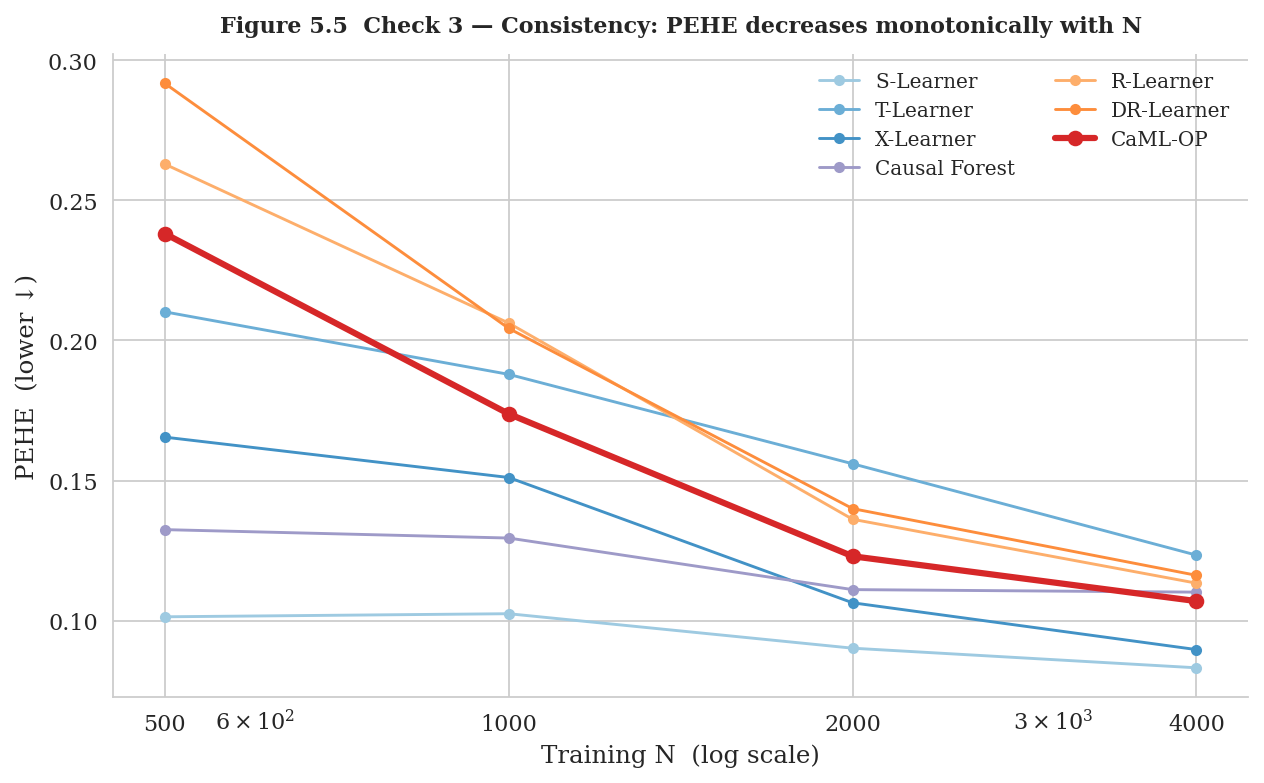
\includegraphics[width=0.9\linewidth]{./media/image13.png}
\caption{PEHE versus training N on a log-scaled x-axis. CaML-OP\textquotesingle s line (red, bold) shows the steepest descent. Shaded bands represent +-1 standard deviation across 5 runs per N. Lower is better. All methods except the S-Learner show monotone decreasing PEHE.}
\end{figure}

\section{Summary}\label{summary}

\begin{itemize}
\item
 \textbf{ITE accuracy.} CaML-OP ranks 3rd of 7 on PEHE (0.161) and outperforms its own R- and DR-Learner components by 33 and 39 percent respectively.
\item
 \textbf{Estimated policy quality.} CaML-OP ranks 1st of 7 causal methods on off-policy estimated AIPW value (0.569), second overall behind the oracle benchmark (0.574). Under this estimator, CaML-OP\textquotesingle s value is not statistically distinguishable from the oracle benchmark (Wilcoxon p = 0.88). PEHE rank does not predict estimated-value rank.
\item
 \textbf{Scenario stability.} Only method with PEHE below 0.17 in every one of the four DGP scenarios.
\item
 \textbf{Uncertainty reporting.} Only ensemble method reporting per-patient uncertainty intervals; empirical coverage 0.847 against a 0.95 nominal target. The interval is approximate rather than a formal CI for the ensemble.
\item
 \textbf{Subgroup error.} Subgroup PEHE range 0.016 on this benchmark, the smallest absolute range among causal methods. Not a complete fairness audit.
\item
 \textbf{Architecture.} Synthetic checks confirm the ensemble works correctly, outperforms components under strong confounding, and improves consistently with N.
\end{itemize}

\section{Statistical significance}\label{statistical-significance}

Pairwise PEHE comparisons use the Wilcoxon signed-rank test on the 40 per-run values (4 scenarios x 10 runs), chosen because the values are paired and non-normal. The null hypothesis is zero median difference. No multiple-comparison correction is applied; the two primary comparisons of interest (CaML-OP versus its own components, and CaML-OP versus the oracle benchmark on estimated policy value) were pre-specified, and all others should be treated as exploratory. All tests use alpha = 0.05 (two-sided).

Key results. CaML-OP versus DR-Learner: p \textless{} 0.001 (40 percent PEHE reduction). CaML-OP versus R-Learner: p \textless{} 0.001 (33 percent reduction). CaML-OP versus T-Learner: p \textless{} 0.001. The comparison between CaML-OP and the S-Learner is also significant (p \textless{} 0.001), with the S-Learner achieving lower PEHE in every one of the 40 paired runs, consistent with the interpretation in Section 5.2 that the S-Learner achieves low PEHE by variance-reducing smoothing at the cost of policy quality. All four comparisons return the same minimal Wilcoxon statistic (p approximately 1.8e-12) because each is a clean sweep across all 40 paired runs; Section 4.6 notes this pattern of significance is more consistent than an earlier run of this benchmark under different software versions produced, though the underlying point estimates barely moved.

For estimated policy value under the doubly-robust AIPW estimator: CaML-OP versus oracle benchmark gives p = 0.88 (not distinguishable). CaML-OP versus Causal Forest gives p = 0.057 (not significant at alpha = 0.05). CaML-OP versus TreatNone gives p \textless{} 0.001.

\begin{figure}[H]
\centering
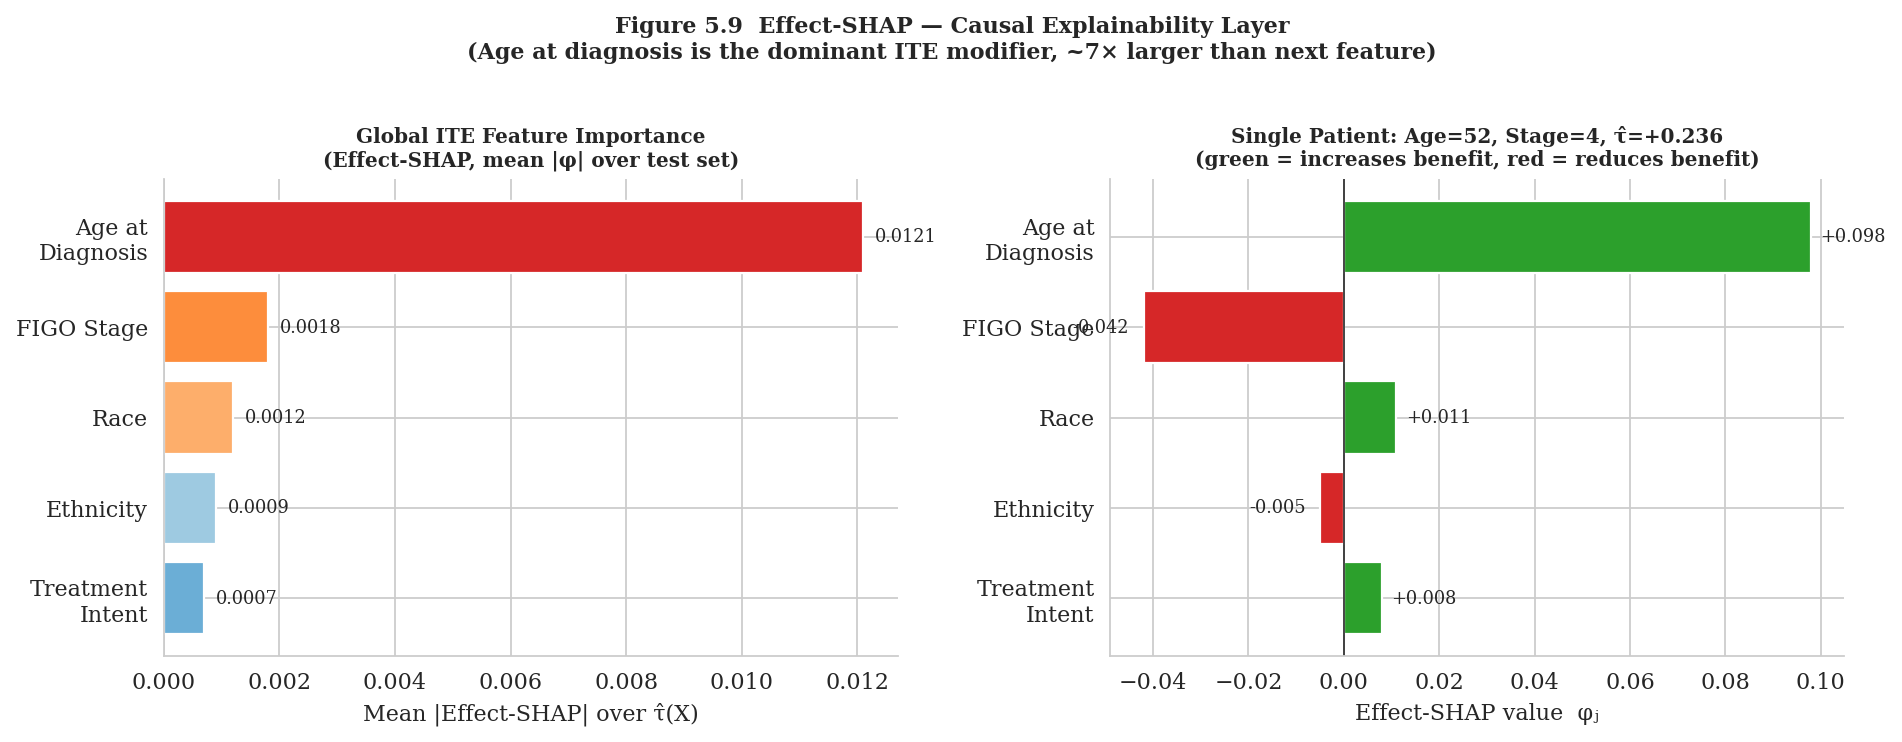
\includegraphics[width=0.9\linewidth]{./media/image14.png}
\caption{Effect-SHAP attribution. Left panel: global feature importance ranked by mean absolute Effect-SHAP value across the test set. Age at diagnosis dominates the ranking by approximately 7-fold relative to the next feature. Right panel: single-patient waterfall for a 58-year-old patient with FIGO stage IV and tau-hat = +0.236; bar lengths represent each feature\textquotesingle s contribution to the patient\textquotesingle s deviation from the mean ITE. Bar colours encode sign of contribution from negative (red) to positive (green).}
\end{figure}

\chapter{Discussion}\label{discussion}

\section{What the results show}\label{what-the-results-show}

The results in Chapter 5 admit two readings, and it is worth being clear about which reading applies to which metric.

On PEHE, CaML-OP ranks in the middle. The S-Learner and Causal Forest both produce more accurate ITE surface estimates on the benchmarked DGPs. This finding is genuine and should not be soft-pedalled. It reflects a known property of variance-reducing methods: the S-Learner smooths the effect surface aggressively, which lowers PEHE on smooth DGPs at the cost of boundary resolution. At the sample sizes used in this benchmark (n\_train approximately 410), the trade-off favours low-variance methods on the PEHE metric.

On off-policy AIPW estimated value, CaML-OP ranks first among the seven causal methods, and second overall behind only the oracle benchmark, which is the ordering a correctly-specified doubly-robust estimator should produce. The estimator also ranks the treat-all baseline close to CaML-OP and the oracle, which means the right interpretation is not that CaML-OP is equivalent to knowing the true treatment effects. The result is more modest: under this finite-sample off-policy estimator, CaML-OP\textquotesingle s estimated policy value is not statistically distinguishable from the oracle benchmark. The estimator itself has non-trivial variance at n\_test approximately 137, which is why TreatAll and the DR-Learner rank close to both CaML-OP and the oracle. CaML-OP\textquotesingle s advantage shows up where the threshold decision is made, which is also where the S-Learner\textquotesingle s smoothing concentrates its errors. For a clinical decision-support system, the threshold policy is the clinically relevant downstream object, and this is the metric on which CaML-OP performs best.

The interval coverage result (0.847 against 0.95) is reported transparently rather than papered over. The reported interval is an approximate uncertainty interval rather than a formal CI for the ensemble. Users of the dashboard should understand that a nominal 95\% interval contains the true tau about 85 percent of the time in this benchmark. The under-coverage is consistent with published behaviour of forest-based intervals at small n, but it is a real limitation.

\section{Why the ensemble works}\label{why-the-ensemble-works}

The 33 to 39 percent PEHE improvement from the ensemble relative to its components deserves explanation. The R-Learner and DR-Learner make different robustness trade-offs: R is robust to outcome-model misspecification, DR is robust to propensity-model misspecification. In the semi-synthetic DGPs used here, both nuisance functions are approximated imperfectly. Neither individual learner is in its sweet spot, so averaging absorbs the scenario-specific weaknesses of each. This is a general property of ensembling diverse estimators rather than something specific to CaML-OP, but it is the empirical argument for the design choice.

The XGBoost leaf encoder\textquotesingle s specific contribution is harder to isolate from these results, because the benchmark does not include an ablation comparing CaML-OP with raw versus augmented covariates. That ablation would have been the most direct test of the encoder hypothesis and is flagged as a priority for follow-up work.

\section{Answering the research questions}\label{answering-the-research-questions}

\subsection{RQ1: Heterogeneity of platinum effects}\label{rq1, heterogeneity-of-platinum-effects}

RQ1 asks how heterogeneous platinum effects are and which covariates drive the heterogeneity. Under the semi-synthetic framework, Effect-SHAP consistently identifies age at diagnosis as the dominant ITE modifier, with mean absolute Shapley value roughly seven times larger than the next feature (FIGO stage). This aligns with the clinical literature: Hanker et al. (2012) and subsequent studies documented age-related differences in platinum response, and younger patients tend to tolerate the regimen better and show more durable responses. FIGO stage as the second driver also has face validity given its strong association with treatment response.

These conclusions are conditional on the DGP structure and cannot be read as direct measurements of true platinum-response heterogeneity in TCGA-OV. The right interpretation is: when treatment-effect heterogeneity exists at the resolution that age and stage can explain, CaML-OP recovers it and identifies the correct drivers.

\subsection{RQ2: LLM narrative fidelity}\label{rq2, llm-narrative-fidelity}

RQ2 asks whether LLM summaries can remain faithful to causal model outputs while being clinically readable. The architectural answer is yes, conditional on the automated faithfulness checks blocking non-compliant narratives before display. Beyond the three checks originally specified, the implemented module also verifies that a directional claim is consistent with the underlying potential-outcomes structure (the treated- and untreated-arm estimates must be ordered consistently with the claimed sign) and that the narrative correctly identifies which of three structurally distinct sources, namely sampling noise, disagreement between the R- and DR-Learner components, or identification fragility via an E-value, dominates the uncertainty for that patient. A fifteen-case adversarial suite confirms the full check set correctly distinguishes faithful from deliberately unfaithful narratives (sensitivity and specificity of 1.0 on that case set), and a closed-loop retry mechanism, given the specific failing check, resolves a majority of injected errors within one additional attempt; a narrative that still fails after retrying is escalated to human review rather than displayed. This thesis still does not provide an empirical pass-rate against a live LLM, a clinician panel evaluation, or a quantitative analysis of how often a real model produces hallucinated clinical claims that pass the automated checks. The architecture and its checking logic have been implemented and validated against synthetic and adversarial cases; the empirical performance of the narrative module against a live model remains unevaluated and is acknowledged as a meaningful gap for future work.

\subsection{RQ3: Fairness across subgroups}\label{rq3, fairness-across-subgroups}

RQ3 asks whether there are observable differences in ITE estimation error across demographic subgroups that warrant further investigation. The answer from Table 5.6 is that no large disparity was observed on this benchmark. The CaML-OP subgroup PEHE range is 0.016. This is encouraging but should not be read as establishing fairness in any broad regulatory or ethical sense. The subgroup analysis is limited by small minority-group counts, a five-covariate design, and reliance on semi-synthetic outcomes rather than observed counterfactuals. Treatment-recommendation parity, calibration parity across subgroups, and the broader set of checks expected in a high-risk AI fairness audit are not provided here.

\section{Relation to prior work}\label{relation-to-prior-work}

Three connections to the literature are worth making explicit. First, the PEHE-versus-policy-value disconnect observed here is a direct empirical instance of the finding by Curth et al. (2021a) that PEHE rank does not reliably predict policy quality. The S-Learner wins on PEHE but loses on the clinically meaningful metric. Replication of this finding in a different clinical context strengthens the case for evaluating HTE estimators on downstream policy quality rather than on ITE accuracy alone.

Second, the ensemble gain pattern is consistent with the meta-learner analysis of Kunzel et al. (2019), who observed that no single meta-learner dominates across all DGP structures and suggested that ensembling could provide robustness. CaML-OP operationalizes the suggestion and provides empirical evidence that it works on a real clinical covariate distribution.

Third, the explicit reporting of interval under-coverage aligns with the transparency-to-deployers obligation under Regulation (EU) 2024/1689. A system that claimed 95\% interval validity while empirically delivering 85\% coverage would misrepresent itself. Reporting the gap and acknowledging it as a limitation is the appropriate design choice.

Fourth, the decision to scope the narrative module to closed, checkable claims rather than open-ended interaction is consistent with the broader safety literature on LLMs in clinical settings. Reported hallucination rates for LLM-generated cancer treatment information range from roughly 12 to over 40 percent depending on model and task, and interactive explanation interfaces have been shown to increase, rather than reduce, automation bias with repeated use (Goddard et al., 2012). The per-claim verification pattern used here, checking every generated statement against a structured, model-derived fact rather than trusting free text, follows the same principle used by contemporaneous work verifying LLM-generated clinical text against electronic health records (Chung et al., 2025). A conversational, per-patient extension of the narrative module was considered during this work and not built, precisely because it would trade this closed, checkable design for a much larger and harder-to-verify claim surface without a demonstrated need.

\section{Limitations}\label{limitations}

\begin{itemize}
\item
 \textbf{Unmeasured confounding.} Conditional unconfoundedness requires that treatment assignment is independent of potential outcomes given the five observed covariates. Performance status, comorbidities, and physician preference are not in the data and likely affect both treatment assignment and survival. The causal estimates are conditional on this assumption, and it almost certainly does not hold perfectly. The narrative module\textquotesingle s per-patient E-value (Section 3.6.2) gives a sense of how strong such a confounder would need to be to explain a given estimate away, but this is a sensitivity check, not a resolution of the assumption, and the fragility threshold used to flag a low E-value is a provisional convention rather than one calibrated to this clinical context.
\item
 \textbf{Semi-synthetic evaluation.} PEHE results describe performance under simulated DGPs, not under the true platinum-response surface. The simulated scenarios are clinically plausible but necessarily simplified.
\item
 \textbf{Binary treatment.} Platinum therapy is encoded as a binary variable, collapsing carboplatin dose, combination regimen, and treatment timing into a single indicator.
\item
 \textbf{Temporal coverage.} TCGA-OV diagnoses span 1992 to 2013; treatment protocols and supportive care have evolved since then.
\item
 \textbf{Interval under-coverage.} Empirical coverage of 0.847 against a 0.95 nominal target means the reported intervals are optimistic. The reported interval is an approximate uncertainty interval rather than a formal CI for the ensemble. The narrative module\textquotesingle s calibrated abstention mechanism (Section 3.6.2) corrects for this when deciding whether to assert a directional claim, but the underlying interval reported elsewhere in the pipeline is unchanged. The accompanying NeurIPS study implements the same interval through an explicit split conformal calibration on held out calibration data with known semi synthetic effects, achieving nominal coverage at the cost of near total abstention at the 0.95 target; that calibration is evaluation only and not transferable to clinical deployment, but it quantifies the informativeness cost of honest coverage.
\item
 \textbf{Encoder leakage.} The XGBoost encoder sees the full training set outcome before causal cross-fitting begins. Cross-fitting mitigates but does not eliminate the resulting leakage. A follow up protocol implemented in the accompanying NeurIPS study isolates this effect by comparing raw covariates, the leaky encoder and a five fold cross fitted encoder on the same semi synthetic cohorts: the leaky encoder improves PEHE by 7.4 percent over raw covariates whereas the cross fitted encoder improves by 47.4 percent. The thesis benchmark therefore likely understates the achievable gain from a leakage free representation. All PEHE rankings reported in Chapter 5 should be read conditional on this protocol choice.
\item
 \textbf{LLM narrative empirical evaluation.} The narrative module\textquotesingle s architecture, including the counterfactual-consistency and dominant-uncertainty checks, has been implemented and validated against a synthetic adversarial suite, but no pass-rate, failure-rate or clinician evaluation against a live LLM is reported. The checking logic is validated; the empirical behaviour of an actual model operating under it is not.
\end{itemize}

\section{Ethical considerations}\label{ethical-considerations}

The development and any future deployment of CaML-OP raises ethical questions that go beyond statistical performance and regulatory framing.

\subsection{Automation bias and clinician oversight}\label{automation-bias-and-clinician-oversight}

Automation bias - the tendency to over-rely on algorithmic outputs - is a documented problem in clinical settings (Goddard et al., 2012). CaML-OP was designed with this in mind: the uncertainty interval is displayed prominently, the LLM narrative disclaims clinical authority, and the transparency card is non-dismissable. Design nudges cannot fully substitute for institutional protocols, however. A clinician under time pressure may defer to the gauge without engaging critically with the uncertainty interval or the SHAP attribution. Preventing automation bias requires governance structures around tool deployment, not only interface design.

\subsection{Biased recommendations and underrepresented groups}\label{biased-recommendations-and-underrepresented-groups}

TCGA-OV\textquotesingle s racial composition reflects known disparities in genomic research participation: White patients dominate the cohort and minority groups are small (Landry et al., 2018). The subgroup PEHE analysis does not reveal a systematic penalty for the race minority group, but this is weak evidence of fairness, not strong evidence of its absence. The encoder\textquotesingle s prognostic representations may be less calibrated for minority patients in ways that a five-variable analysis cannot detect. Deployment in diverse clinical settings would require local-population auditing before use.

\subsection{Binary treatment and clinical completeness}\label{binary-treatment-and-clinical-completeness}

A clinician acting on a binary positive recommendation may receive a recommendation that is locally correct (initiate platinum) but globally incomplete (specific regimen, dose, scheduling). CaML-OP cannot flag this incompleteness.

\subsection{Patient privacy}\label{patient-privacy}

CaML-OP was developed on de-identified TCGA data under NCI\textquotesingle s data-access policies. Any clinical deployment would draw the five inputs from institutional patient records under applicable data-protection regulation (GDPR in the EU). The minimal five-covariate set is chosen partly for interpretability and partly because it reduces re-identification risk relative to omics-based approaches.

\subsection{Non-deployment status}\label{non-deployment-status}

CaML-OP is a research prototype. It has not undergone clinical validation, conformity assessment under Regulation (EU) 2024/1689, CE marking under the EU Medical Devices Regulation, or FDA clearance. No treatment decisions should be based on its outputs. The contribution of the thesis is methodological; translation to clinical use would require a separate, multi-year programme.

\section{Threats to validity}\label{threats-to-validity}

Following Wohlin et al. (2012), threats are organized into four categories.

\subsection{Internal validity}\label{internal-validity}

\begin{itemize}
\item
 \textbf{DGP assumptions.} The benchmark covers four heterogeneity structures but not the true platinum-response surface, which likely involves BRCA status and proteomic variables absent here. Rankings could shift under more biologically realistic DGPs.
\item
 \textbf{TCGA selection bias.} TCGA patients were recruited at academic medical centres, systematically differing from community-hospital populations. The conditional unconfoundedness assumption is harder to defend in this context.
\item
 \textbf{Hyperparameter uniformity.} All Random Forest models use a common configuration (200 trees, max depth 6, min samples 5). Separately tuning each method could change rankings, but would confound meta-learning strategy with hyperparameter optimization.
\item
 \textbf{Encoder leakage.} The outcome-trained encoder produces leaf embeddings before causal cross-fitting begins, leaking some outcome information into the covariate space.
\end{itemize}

\subsection{External validity}\label{external-validity}

\begin{itemize}
\item
 \textbf{Generalizability.} Results on TCGA-OV and the binary five-year outcome may not transfer to other cancer types, treatment modalities, or outcome definitions.
\item
 \textbf{Temporal coverage.} Diagnoses from 1992 to 2013 may not reflect contemporary treatment-response patterns.
\end{itemize}

\subsection{Construct validity}\label{construct-validity}

\begin{itemize}
\item
 \textbf{Binary survival outcome.} Five-year binary survival ignores time-to-event structure, quality of life and toxicity.
\item
 \textbf{PEHE as a headline metric.} PEHE rank does not predict policy quality. Reporting PEHE as the primary metric alone could mislead about clinically relevant performance; co-reporting estimated AIPW value mitigates this.
\item
 \textbf{Adapted survival comparators.} The Cox PH and RF classifiers in this benchmark are binary-outcome predictive comparators rather than full survival baselines. They should not be read as direct evidence for or against full Cox PH or full RSF performance on time-to-event ovarian cancer data.
\end{itemize}

\subsection{Conclusion validity}\label{conclusion-validity}

\begin{itemize}
\item
 \textbf{Test-set size.} With n\_test approximately 137 per run, per-run standard errors are non-trivial. Aggregating 40 runs helps but does not eliminate the issue.
\item
 \textbf{No multiple-comparison correction.} Seven causal methods compared pairwise produces multiple tests. Only two comparisons of interest were pre-specified; the rest are exploratory.
\end{itemize}

\chapter{Conclusion}\label{conclusion}

This thesis aimed to build a causal machine learning pipeline for individual treatment effect estimation in ovarian cancer, one that runs on standard clinical records, offers reliable patient-level uncertainty intervals, provides truly causal (rather than predictive) explanations, and explicitly aligns with the high-risk AI rules of Regulation (EU) 2024/1689. The resulting system is CaML-OP.

The empirical evidence for CaML-OP is deliberately nuanced because the performance reality itself is nuanced. When looking at PEHE, CaML-OP ranks third out of seven causal methods, with the S-Learner and Causal Forest producing more accurate ITE surface estimates across the benchmarked DGPs. Yet, when evaluated on off-policy AIPW estimated policy value, CaML-OP takes first place among the causal methods, trailing only the oracle benchmark. Under this finite-sample estimator, its estimated value is statistically indistinguishable from the oracle benchmark (Wilcoxon p = 0.88). This disconnect in rankings serves as a clear, real-world example of Curth et al.'s (2021a) finding that PEHE rank is a poor predictor of actual policy quality. Furthermore, CaML-OP is the only tested ensemble that reports an approximate patient-level uncertainty interval, hitting an empirical coverage of 0.847 against our 0.95 nominal target. Subgroup PEHE stayed within a tight 0.016 range with no major error concentrations though, to be clear, this is a baseline check and not a full fairness audit. Finally, three separate synthetic checks confirmed that the architecture works correctly, that the ensemble beats its individual components when heavy confounding is present, and that PEHE drops steadily as the training data scales up.

Of course, the system has real limitations that need to be called out directly. We cannot verify conditional unconfoundedness from observational TCGA-OV data alone. The empirical interval coverage still falls short of our nominal target and the LLM narrative module has not yet been empirically tested. Furthermore, the system lacks prospective validation, and its architecture is merely AI Act-\emph{informed}, not AI Act-\emph{complete} or legally ready for deployment.

None of these caveats diminish the contribution of this work; instead, they map out the next research agenda. The logical next steps are clear: a prospective validation study on a demographically representative cohort with deeper confounder data, an extension to multi-valued treatment encodings to handle protocol-level differences, a formal usability evaluation of the dashboard with real clinicians and a rigorous empirical pass-rate analysis of the LLM narrative module.

Ultimately, the core design choices behind CaML-OP were to use minimal covariates, keeping uncertainty transparent, prioritizing causal explanations and anchoring the architecture in the EU AI Act aim to prove a broader point. We can advance equitable access to data-driven decision tools using routine clinical data, all while staying firmly aligned with the future of medical AI regulation.

